\documentclass[aspectratio=169, 10pt]{beamer}

% --- THEME & COLOR CONFIGURATION ---
\usetheme{Madrid}
\useinnertheme{rectangles}

\definecolor{hcmutnavy}{RGB}{11, 42, 74}
\definecolor{hcmutblue}{RGB}{23, 105, 170}
\definecolor{hcmutcyan}{RGB}{22, 166, 182}
\definecolor{hcmutdark}{RGB}{23, 50, 77}
\definecolor{hcmutlight}{RGB}{247, 251, 255}
\definecolor{hcmutgreen}{RGB}{46, 125, 50}
\definecolor{hcmutred}{RGB}{198, 40, 40}

\setbeamercolor{palette primary}{bg=hcmutnavy, fg=white}
\setbeamercolor{palette secondary}{bg=hcmutblue, fg=white}
\setbeamercolor{palette tertiary}{bg=hcmutcyan, fg=white}
\setbeamercolor{palette quaternary}{bg=hcmutdark, fg=white}

\setbeamercolor{structure}{fg=hcmutblue}
\setbeamercolor{titlelike}{parent=palette primary}
\setbeamercolor{block title}{bg=hcmutblue, fg=white}
\setbeamercolor{block body}{bg=hcmutlight, fg=hcmutdark}
\setbeamercolor{block title example}{bg=hcmutcyan, fg=white}
\setbeamercolor{block body example}{bg=hcmutlight, fg=hcmutdark}

\setbeamertemplate{navigation symbols}{}
\setbeamertemplate{footline}{
  \leavevmode%
  \hbox{%
    \begin{beamercolorbox}[wd=.333333\paperwidth,ht=2.25ex,dp=1ex,center]{author in head/foot}%
      \usebeamerfont{author in head/foot}\textbf{Hoàng Trọng Huy Minh} (2452743)
    \end{beamercolorbox}%
    \begin{beamercolorbox}[wd=.333333\paperwidth,ht=2.25ex,dp=1ex,center]{title in head/foot}%
      \usebeamerfont{title in head/foot}CO3133: Deep Learning — Assignment 1
    \end{beamercolorbox}%
    \begin{beamercolorbox}[wd=.333333\paperwidth,ht=2.25ex,dp=1ex,right]{date in head/foot}%
      \usebeamerfont{date in head/foot}Group Goat \hspace*{2em}
      \insertframenumber{} / \inserttotalframenumber\hspace*{2ex}
    \end{beamercolorbox}%
  }%
  \vskip0pt%
}

% --- PACKAGES ---
\usepackage{booktabs}
\usepackage{amsmath, amssymb}
\usepackage{graphicx}
\usepackage{hyperref}
\usepackage{array}
\usepackage{colortbl}

\hypersetup{colorlinks=true, linkcolor=hcmutblue, urlcolor=hcmutcyan}

% --- METADATA ---
\title[\textbf{Assignment 1: Deep Learning Architectures}]{\textbf{Foundations of Deep Learning Pipelines \& Architectures}}
\subtitle{From Linear Models to Modern Sequence Models: A Comparative Study for Image Classification}
\author[\textbf{Hoàng Trọng Huy Minh}]{\textbf{Hoàng Trọng Huy Minh} (Student ID: 2452743) \\ \small\textbf{100\% Sole Contributor} \quad (\textit{Other Members: 0\%})}
\institute[HCMUT]{
  \textbf{Faculty of Computer Science and Engineering} \\
  \textbf{Ho Chi Minh City University of Technology (HCMUT) — VNU-HCM} \\
  \vspace{0.2em}
  Course: \textbf{CO3133: Deep Learning and Its Applications (Semester 261)} \\
  Instructor: \textbf{Assoc. Prof. Lê Thành Sách}
}
\date{Group Goat — October 2026}

\begin{document}

% =========================================================================
% SLIDE 1: TITLE SLIDE
% =========================================================================
\begin{frame}[plain]
  \begin{columns}[c]
    \begin{column}{0.72\textwidth}
      \titlepage
    \end{column}
    \begin{column}{0.25\textwidth}
      \centering
      
\includegraphics[width=0.65\linewidth, keepaspectratio]{hcmut_logo.png}
      \vspace{0.8em}
      \begin{block}{\centering \footnotesize Group Goat}
        \centering\scriptsize
        \textbf{Lead Author:}\\
        Hoàng Trọng Huy Minh\\
        (100\% Contribution)
      \end{block}
    \end{column}
  \end{columns}
\end{frame}

% =========================================================================
% SLIDE 2: PRESENTATION OUTLINE
% =========================================================================
\begin{frame}{\textbf{Presentation Agenda \& Navigation}}
  \begin{columns}[t]
    \begin{column}{0.48\textwidth}
      \begin{block}{\textbf{Part I: Foundations \& Data Pipeline}}
        \begin{itemize}\footnotesize
          \item Real-World Motivation \& Task Formulation
          \item Fashion-MNIST Exploratory Data Analysis (EDA)
          \item Stratified Splitting \& Leakage Prevention
          \item Unified Optimization \& Evaluation Protocols
        \end{itemize}
      \end{block}
      \vspace{0.3em}
      \begin{block}{\textbf{Part II: Baseline Architectures (M1)}}
        \begin{itemize}\footnotesize
          \item Linear / Softmax Regression Classifier
          \item Multilayer Perceptron (MLP) with Regularization
        \end{itemize}
      \end{block}
    \end{column}
    \begin{column}{0.48\textwidth}
      \begin{block}{\textbf{Part III: Modern Architectures (M2)}}
        \begin{itemize}\footnotesize
          \item Custom 3-Stage Convolutional Neural Network
          \item Bidirectional LSTM for Sequential Image Scans
          \item Vision Transformer (ViT) with Self-Attention
        \end{itemize}
      \end{block}
      \vspace{0.3em}
      \begin{block}{\textbf{Part IV: Benchmark, Errors \& Compliance}}
        \begin{itemize}\footnotesize
          \item Master 5-Model Comparative Benchmark
          \item Error Taxonomy \& Qualitative Visualizations
          \item Inductive Bias vs Capacity Trade-offs
          \item Automated Sanity Audits \& AI Disclosures
        \end{itemize}
      \end{block}
    \end{column}
  \end{columns}
\end{frame}

% =========================================================================
% SLIDE 3: PROBLEM FORMULATION
% =========================================================================
\begin{frame}{\textbf{Problem Formulation: Beyond Digit Recognition}}
  \begin{columns}[c]
    \begin{column}{0.58\textwidth}
      \begin{block}{\textbf{Task Definition \& Formulation}}
        \scriptsize
        Given a grayscale apparel image $\mathbf{x} \in [0, 1]^{28 \times 28}$, predict class label $y \in \{0, 1, \dots, 9\}$:
        $$\hat{y} = \arg\max_{c \in \{0, \dots, 9\}} p(y = c \mid \mathbf{x}; \boldsymbol{\theta})$$
      \end{block}
      \vspace{0.2em}
      \begin{block}{\textbf{Key Technical Challenges in Fashion-MNIST}}
        \begin{itemize}\scriptsize
          \item \textbf{High Intra-Class Variance}: Diverse fabric styles, cuts, and sleeve lengths within classes.
          \item \textbf{Subtle Inter-Class Ambiguity}: Close morphology between \textit{T-shirt}, \textit{Shirt}, and \textit{Coat}.
          \item \textbf{Low Resolution}: Only $28 \times 28$ pixels without RGB color channels or fine textures.
        \end{itemize}
      \end{block}
    \end{column}
    \begin{column}{0.38\textwidth}
      \centering
      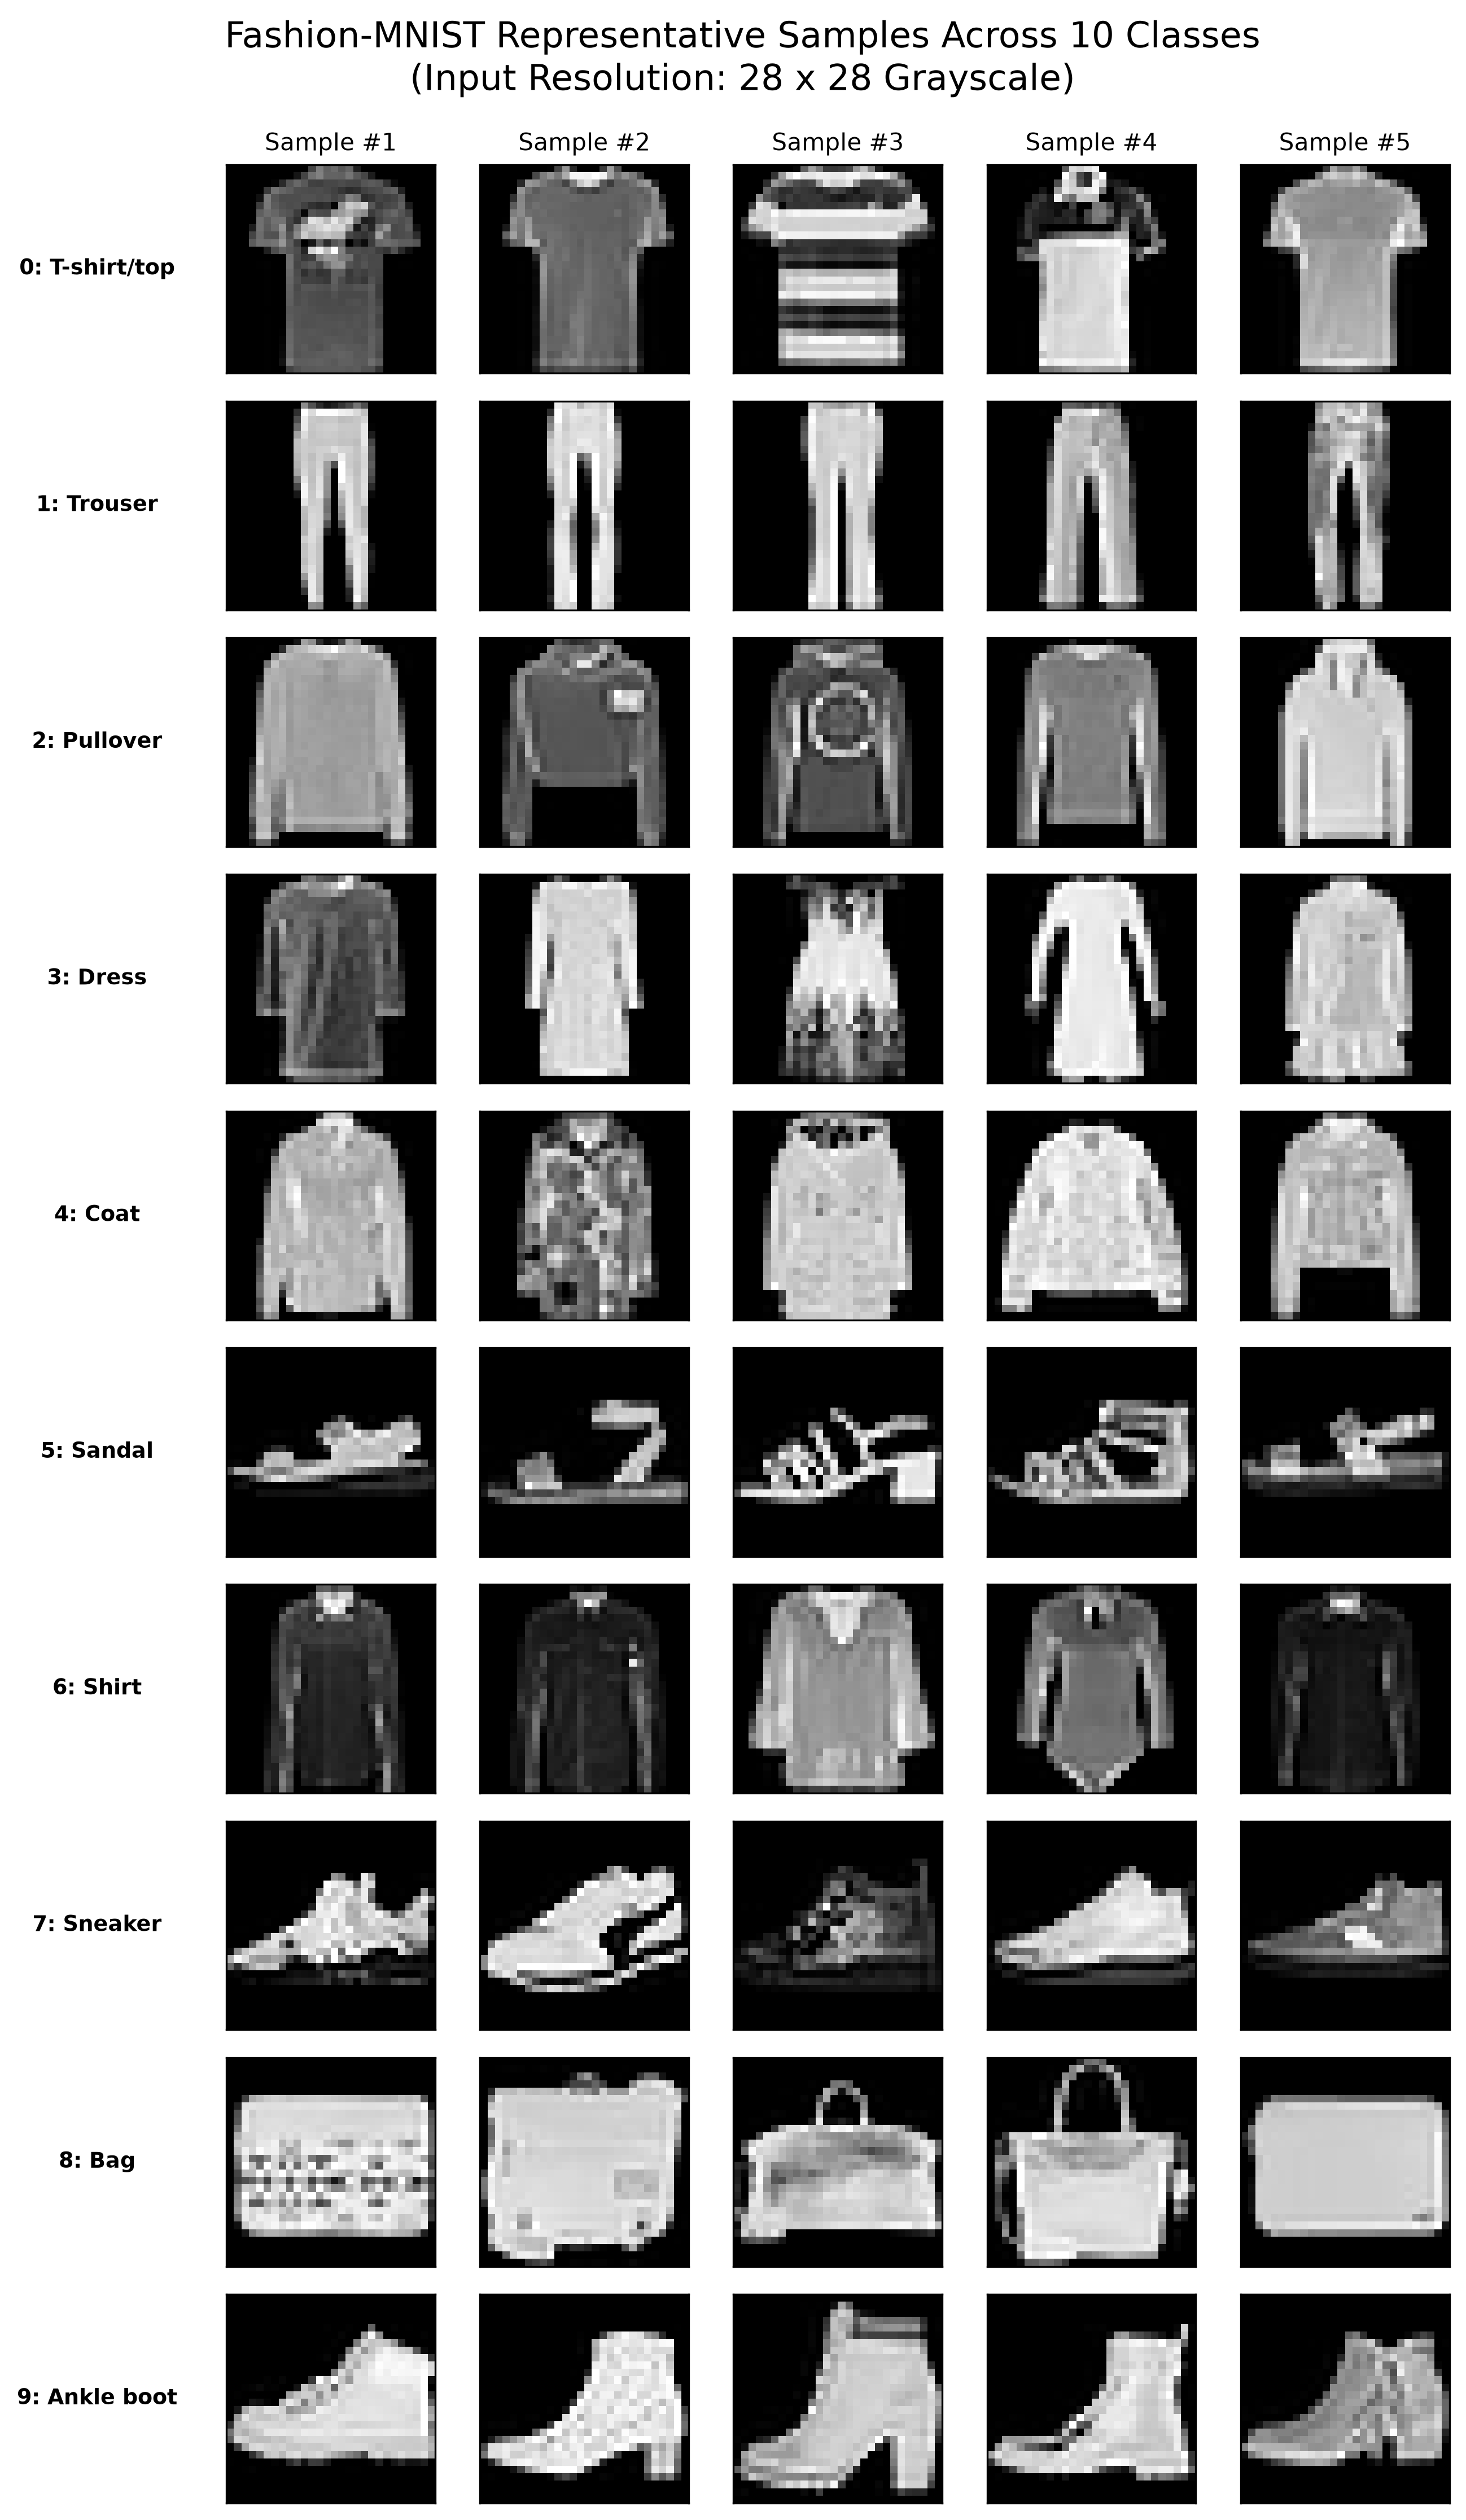
\includegraphics[width=\linewidth, height=0.62\textheight, keepaspectratio]{eda_figures/fig1_representative_samples.png}
      \vspace{0.2em}
      {\tiny \textbf{Figure 1:} Fashion-MNIST apparel samples.}
    \end{column}
  \end{columns}
\end{frame}

% =========================================================================
% SLIDE 4: EXPLORATORY DATA ANALYSIS (EDA)
% =========================================================================
\begin{frame}{\textbf{Exploratory Data Analysis: Distributions \& Projections}}
  \begin{columns}[c]
    \begin{column}{0.48\textwidth}
      \centering
      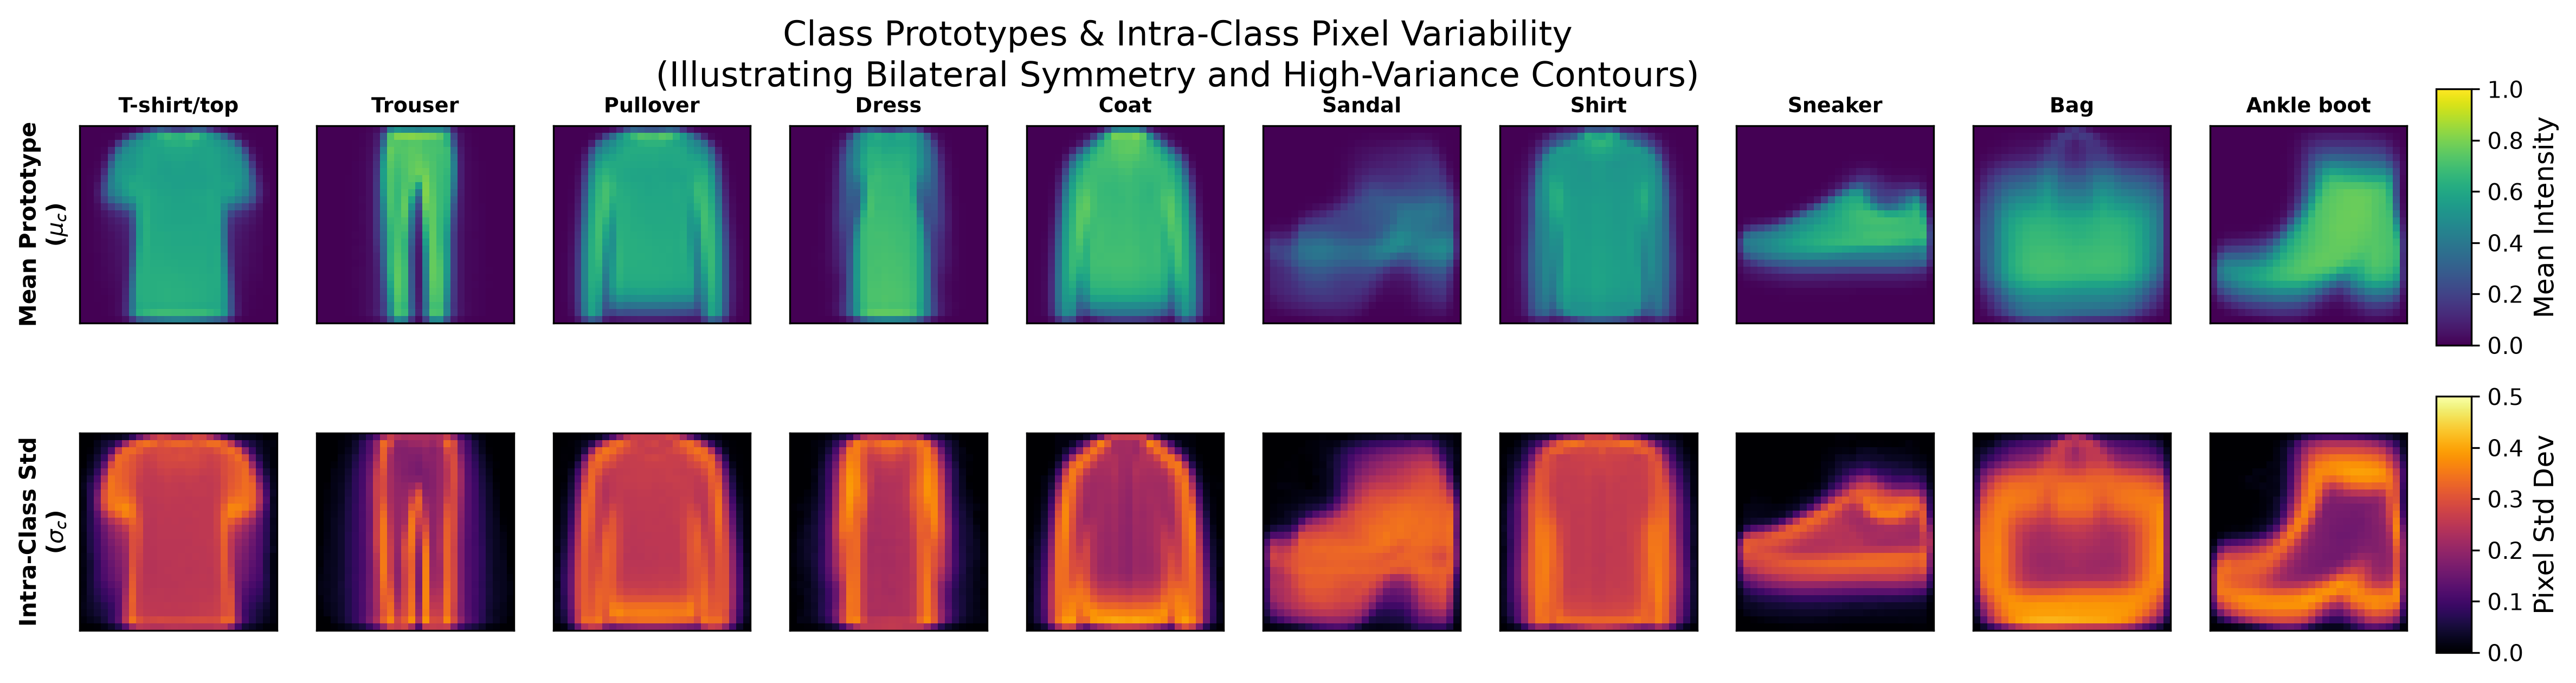
\includegraphics[width=\linewidth, height=0.40\textheight, keepaspectratio]{eda_figures/fig4_class_prototypes.png}
      \vspace{0.2em}
      \begin{block}{\textbf{Class Prototypes (Mean $\pm$ Std)}}
        \scriptsize
        Mean images reveal central mass concentration for tops vs bifurcated legs for \textit{Trouser} and sole geometry for footwear.
      \end{block}
    \end{column}
    \begin{column}{0.48\textwidth}
      \centering
      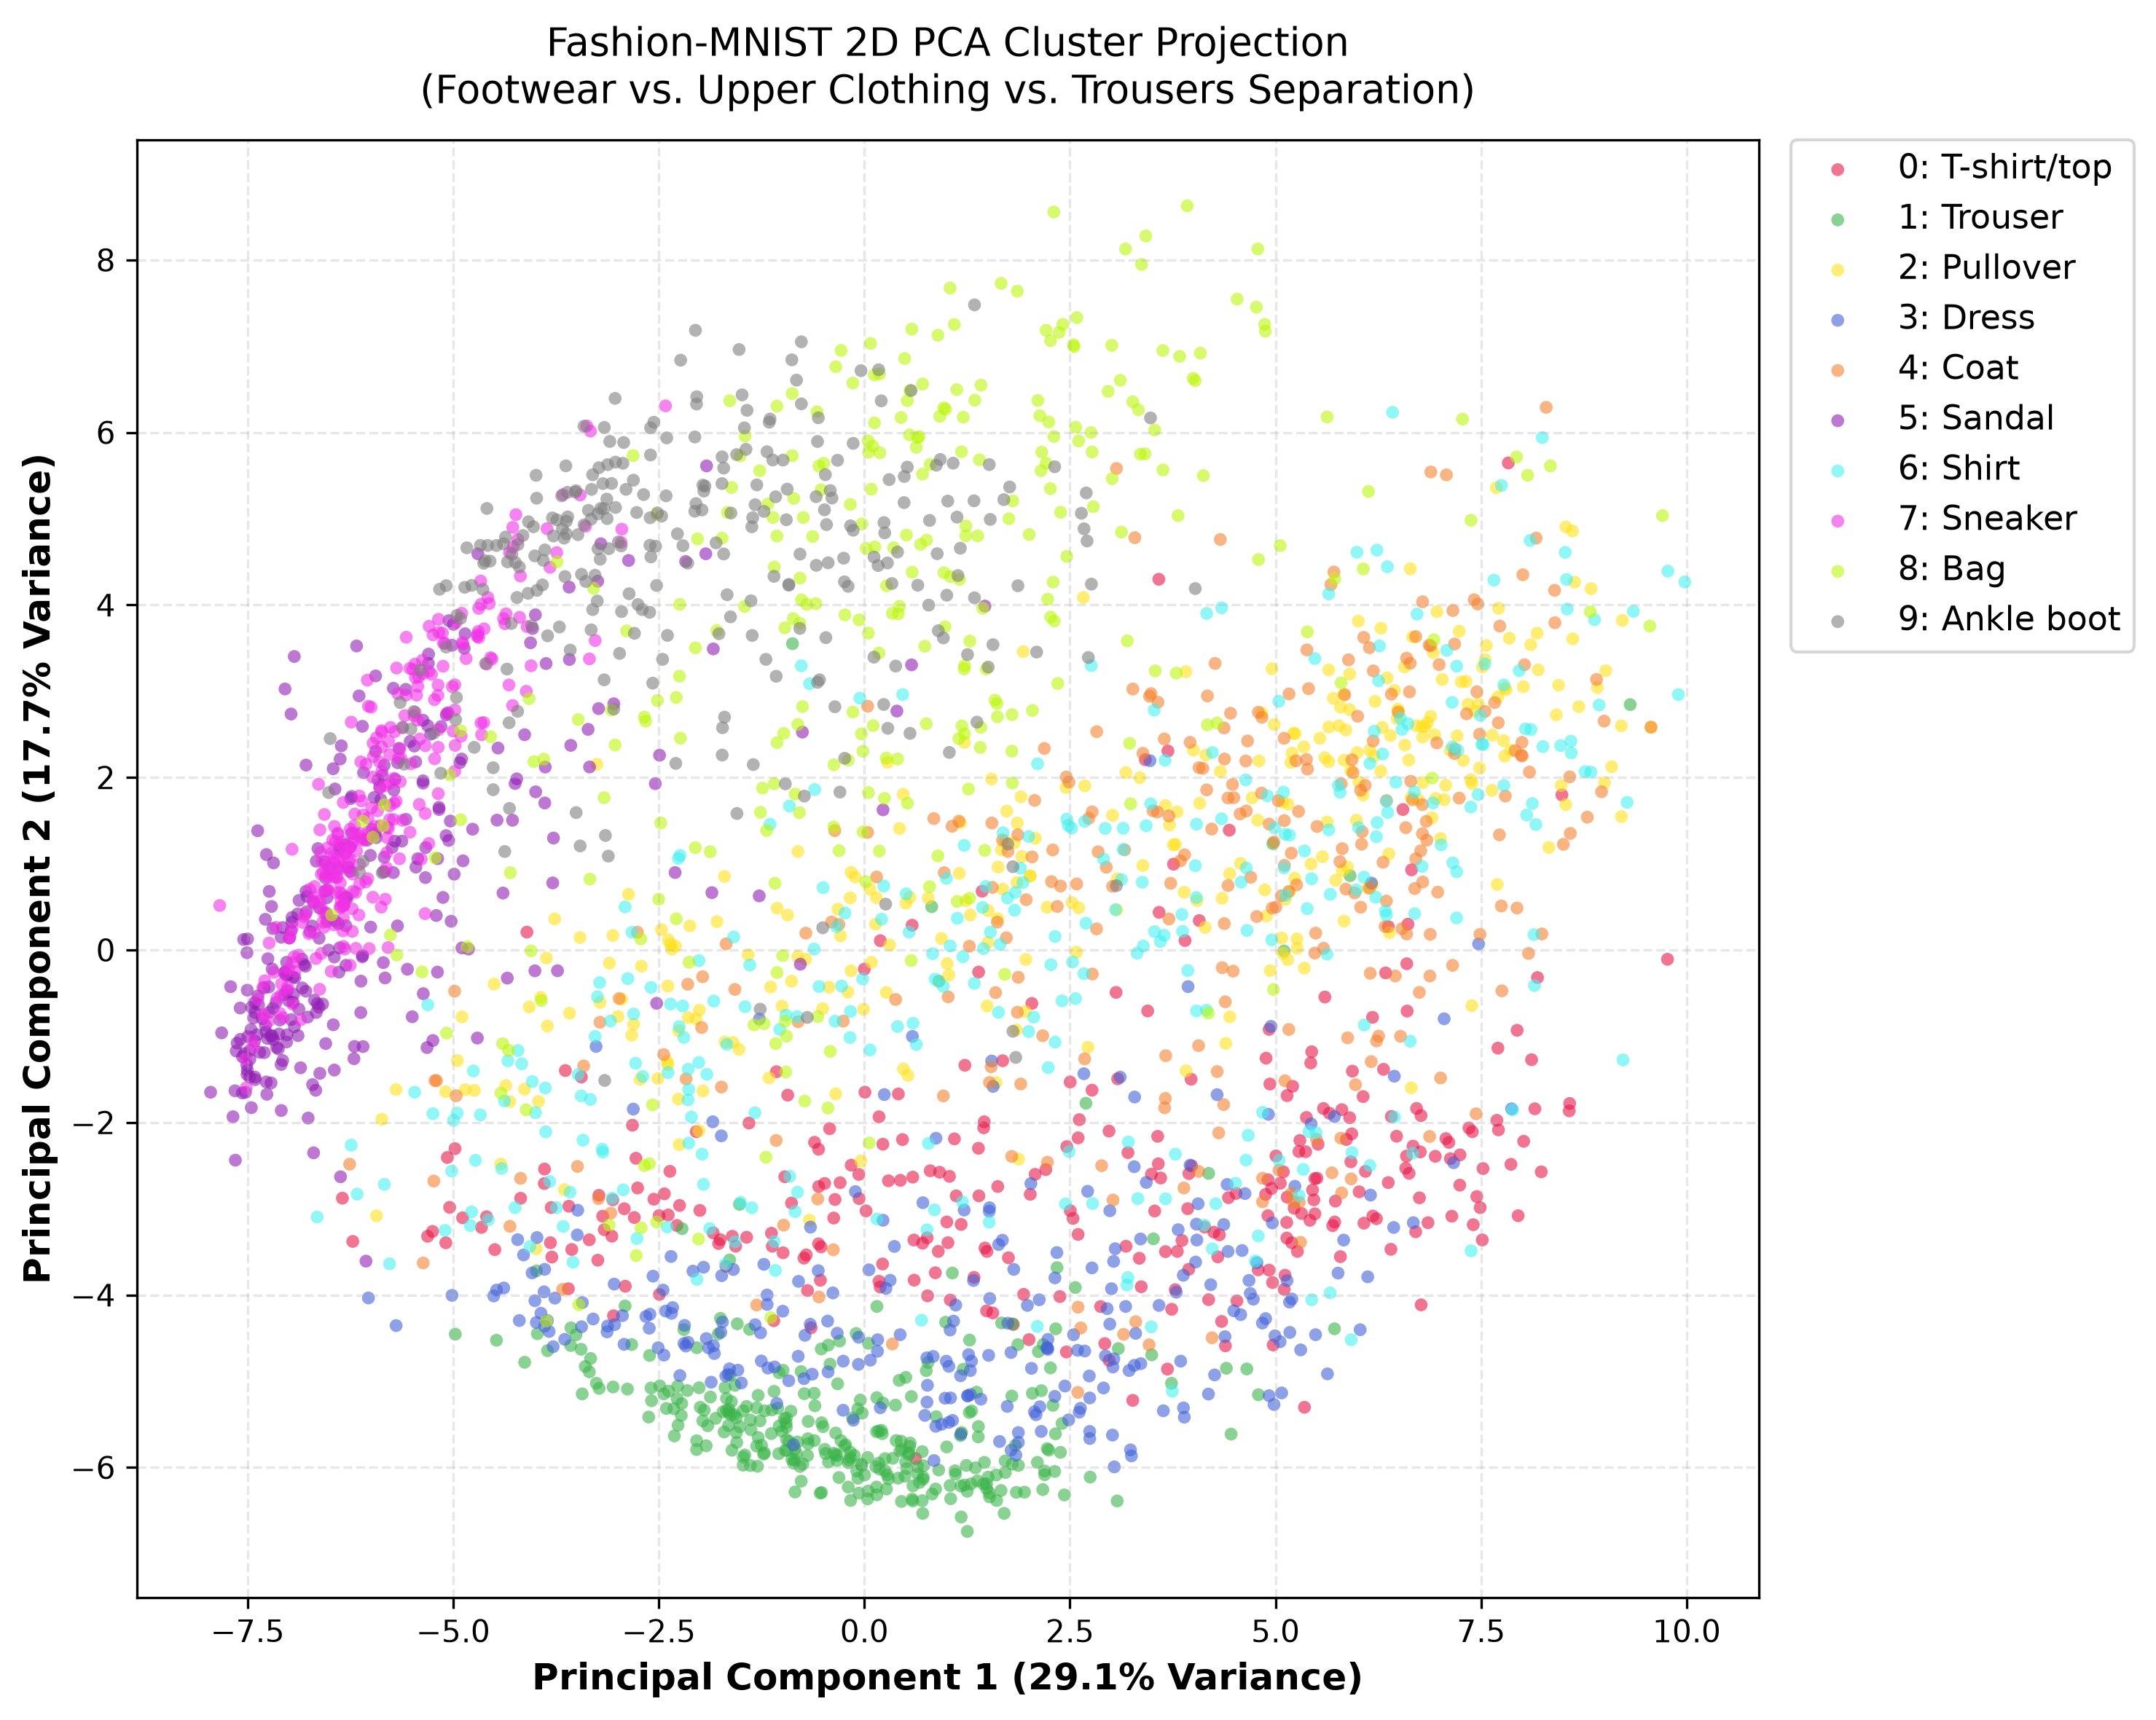
\includegraphics[width=0.82\linewidth, height=0.45\textheight, keepaspectratio]{eda_figures/fig5_pca_clusters.png}
      \vspace{0.2em}
      \begin{block}{\textbf{2D PCA Manifold Projection}}
        \scriptsize
        Footwear and \textit{Trouser} form isolated clusters; upper garments (\textit{Shirt}, \textit{Coat}, \textit{Pullover}) heavily overlap in linear space.
      \end{block}
    \end{column}
  \end{columns}
\end{frame}

% =========================================================================
% SLIDE 5: UNIFIED PIPELINE & FAIRNESS PROTOCOL
% =========================================================================
\begin{frame}{\textbf{Leakage-Free Pipeline \& Experimental Fairness}}
  \begin{columns}[c]
    \begin{column}{0.50\textwidth}
      \begin{block}{\textbf{Rigorous Stratified Partition (Seed 42)}}
        \begin{itemize}\scriptsize
          \item \textbf{Training Set}: 50,000 samples (5,000 / class)
          \item \textbf{Validation Set}: 10,000 samples (1,000 / class)
          \item \textbf{Test Set}: 10,000 samples (1,000 / class)
          \item \textbf{Leakage Prevention}: Instance-level isolation; zero sample intersection ($\mathcal{S}_{\text{train}} \cap \mathcal{S}_{\text{val}} = \emptyset$).
        \end{itemize}
      \end{block}
      \vspace{0.3em}
      \begin{block}{\textbf{Feature Normalization}}
        \scriptsize
        Channel normalized using dataset statistics:
        $$\tilde{x} = \frac{x - \mu}{\sigma}, \quad \mu = 0.2860, \; \sigma = 0.3530$$
      \end{block}
    \end{column}
    \begin{column}{0.46\textwidth}
      \begin{block}{\textbf{Unified Training Configuration}}
        \begin{itemize}\scriptsize
          \item \textbf{Batch Size}: 64
          \item \textbf{Optimizer}: AdamW ($\beta_1=0.9, \beta_2=0.999$)
          \item \textbf{Initial Learning Rate}: $\eta_0 = 10^{-3}$
          \item \textbf{Weight Decay}: $\lambda = 10^{-4}$
          \item \textbf{Learning Rate Schedule}: Cosine Annealing:
          $$\eta_t = \eta_{\min} + \frac{1}{2}(\eta_0 - \eta_{\min})\left(1 + \cos\frac{\pi t}{T_{\max}}\right)$$
          \item \textbf{Checkpoint Criterion}: Best Validation Macro-F1 (patience = 4 epochs).
          \item \textbf{Hardware}: NVIDIA GeForce RTX 3060.
        \end{itemize}
      \end{block}
    \end{column}
  \end{columns}
\end{frame}

% =========================================================================
% SLIDE 6: M1 BASELINE — LINEAR CLASSIFIER
% =========================================================================
\begin{frame}{\textbf{M1 Baseline: Linear / Softmax Regression Classifier}}
  \begin{columns}[c]
    \begin{column}{0.52\textwidth}
      \begin{block}{\textbf{Mathematical Formulation}}
        \scriptsize
        Flattens $\mathbf{x} \in \mathbb{R}^{28 \times 28}$ to vector $\mathbf{v} \in \mathbb{R}^{784}$:
        $$\mathbf{z} = \mathbf{W}\mathbf{v} + \mathbf{b}, \quad \mathbf{W} \in \mathbb{R}^{10 \times 784}, \; \mathbf{b} \in \mathbb{R}^{10}$$
        $$p(y = c \mid \mathbf{x}) = \frac{\exp(z_c)}{\sum_{j=0}^9 \exp(z_j)}$$
        Loss: PyTorch \texttt{CrossEntropyLoss} operates on raw logits $\mathbf{z}$ (\textbf{no premature softmax applied}).
      \end{block}
      \vspace{0.2em}
      \begin{block}{\textbf{Empirical Results \& Structural Limitation}}
        \begin{itemize}\scriptsize
          \item \textbf{Trainable Parameters}: $784 \times 10 + 10 = \mathbf{7{,}850}$
          \item \textbf{Test Accuracy}: $\mathbf{84.49\%}$ \quad \textbf{Test Macro-F1}: $\mathbf{84.37\%}$
          \item \textbf{Structural Bottleneck}: Separating hyperplanes cannot isolate concave manifolds or complex garment textures.
        \end{itemize}
      \end{block}
    \end{column}
    \begin{column}{0.45\textwidth}
      \centering
      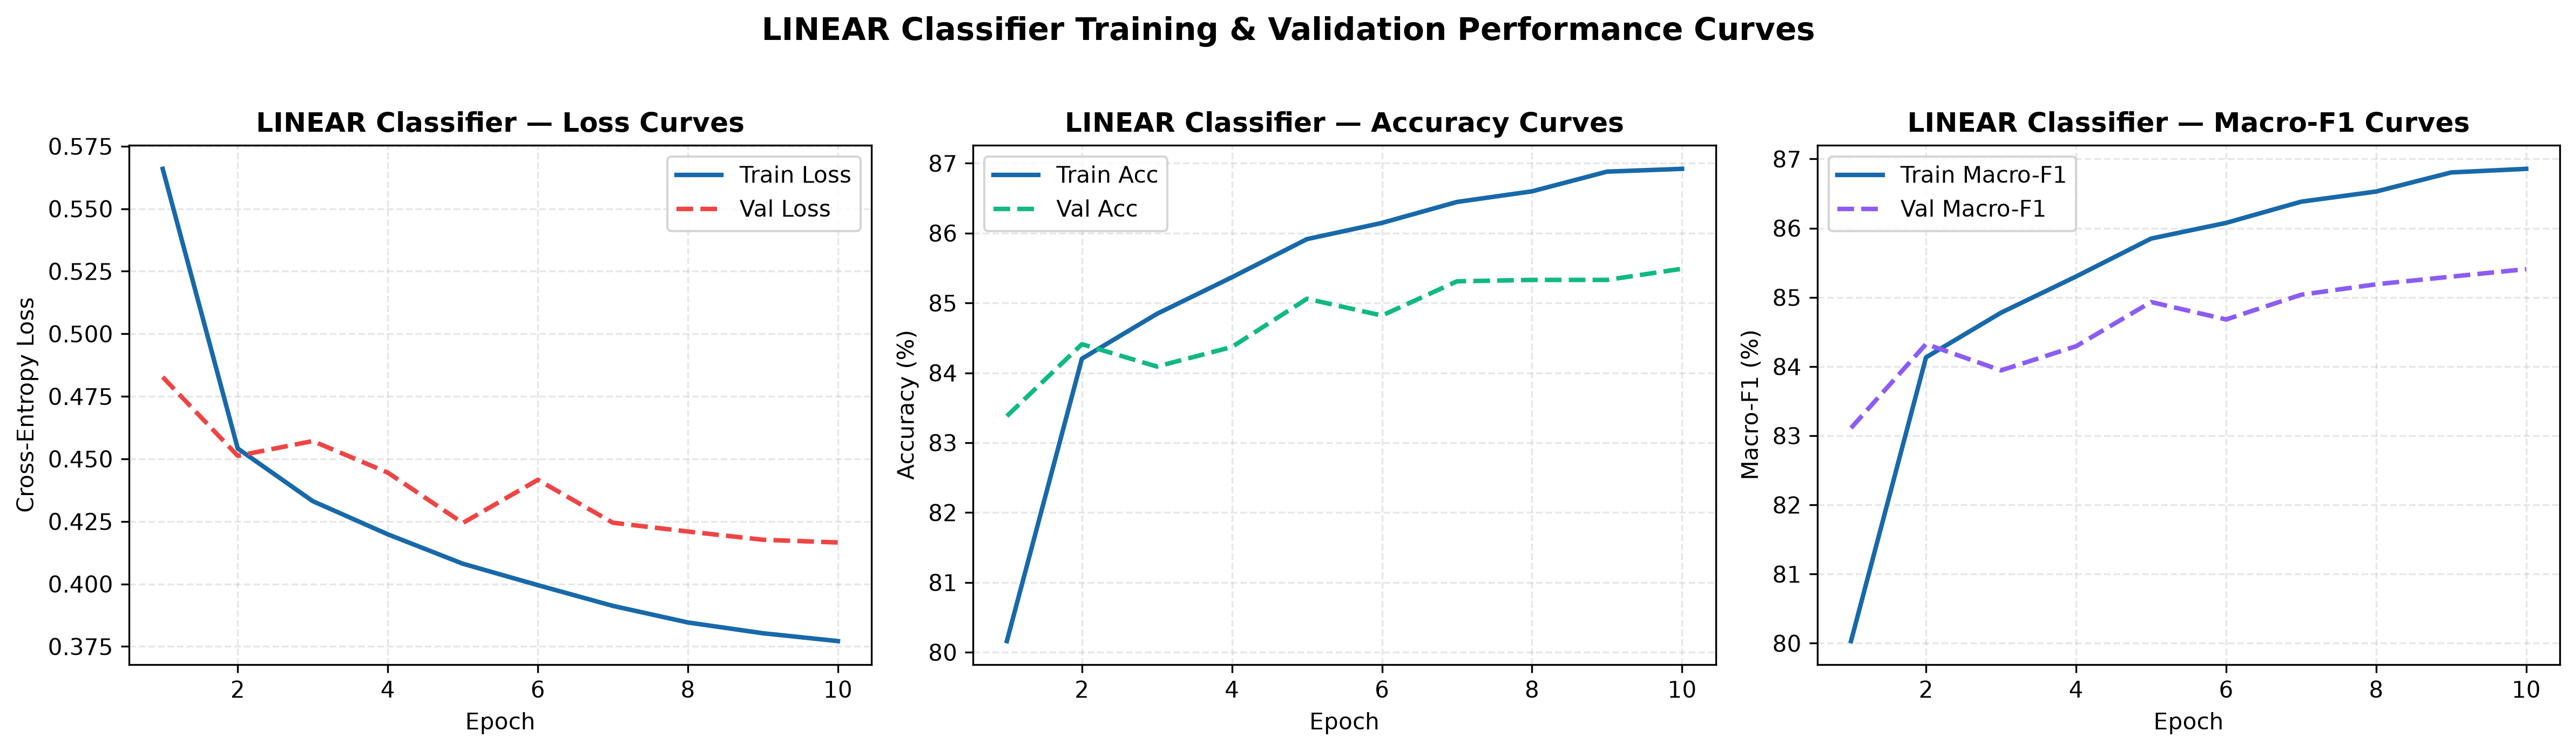
\includegraphics[width=\linewidth, height=0.38\textheight, keepaspectratio]{outputs/figures/learning_curves_linear.png}
      \vspace{0.2em}
      {\tiny \textbf{Figure 2:} Training and validation dynamics for Linear model.}
      \vspace{0.3em}
      \begin{block}{\textbf{Convergence Observation}}
        \scriptsize
        Rapid plateau after epoch 3; validation accuracy asymptotes at $84.5\%$.
      \end{block}
    \end{column}
  \end{columns}
\end{frame}

% =========================================================================
% SLIDE 7: M1 BASELINE — MULTILAYER PERCEPTRON (MLP)
% =========================================================================
\begin{frame}{\textbf{M1 Baseline: Multilayer Perceptron (MLP)}}
  \begin{columns}[c]
    \begin{column}{0.52\textwidth}
      \begin{block}{\textbf{Architecture \& Non-Linear Representation}}
        \scriptsize
        Hierarchical non-linear projections with intermediate normalization and stochastic regularization:
        $$\mathbf{h}_1 = \text{Dropout}_{0.2}(\text{ReLU}(\text{BN}(\mathbf{W}_1\mathbf{v} + \mathbf{b}_1)))$$
        $$\mathbf{h}_2 = \text{Dropout}_{0.2}(\text{ReLU}(\text{BN}(\mathbf{W}_2\mathbf{h}_1 + \mathbf{b}_2)))$$
        $$\mathbf{z} = \mathbf{W}_3\mathbf{h}_2 + \mathbf{b}_3$$
        Dimensions: $784 \to 256 \to 128 \to 10$.
      \end{block}
      \vspace{0.2em}
      \begin{block}{\textbf{Empirical Results \& Trade-offs}}
        \begin{itemize}\scriptsize
          \item \textbf{Parameters}: $\mathbf{235{,}146}$ ($\sim 30\times$ more than Linear).
          \item \textbf{Test Accuracy}: $\mathbf{88.86\%}$ ($+4.37\%$ gain over Linear).
          \item \textbf{Inductive Limitation}: Treats pixels as an unordered bag of features; destroys 2D spatial locality.
        \end{itemize}
      \end{block}
    \end{column}
    \begin{column}{0.45\textwidth}
      \centering
      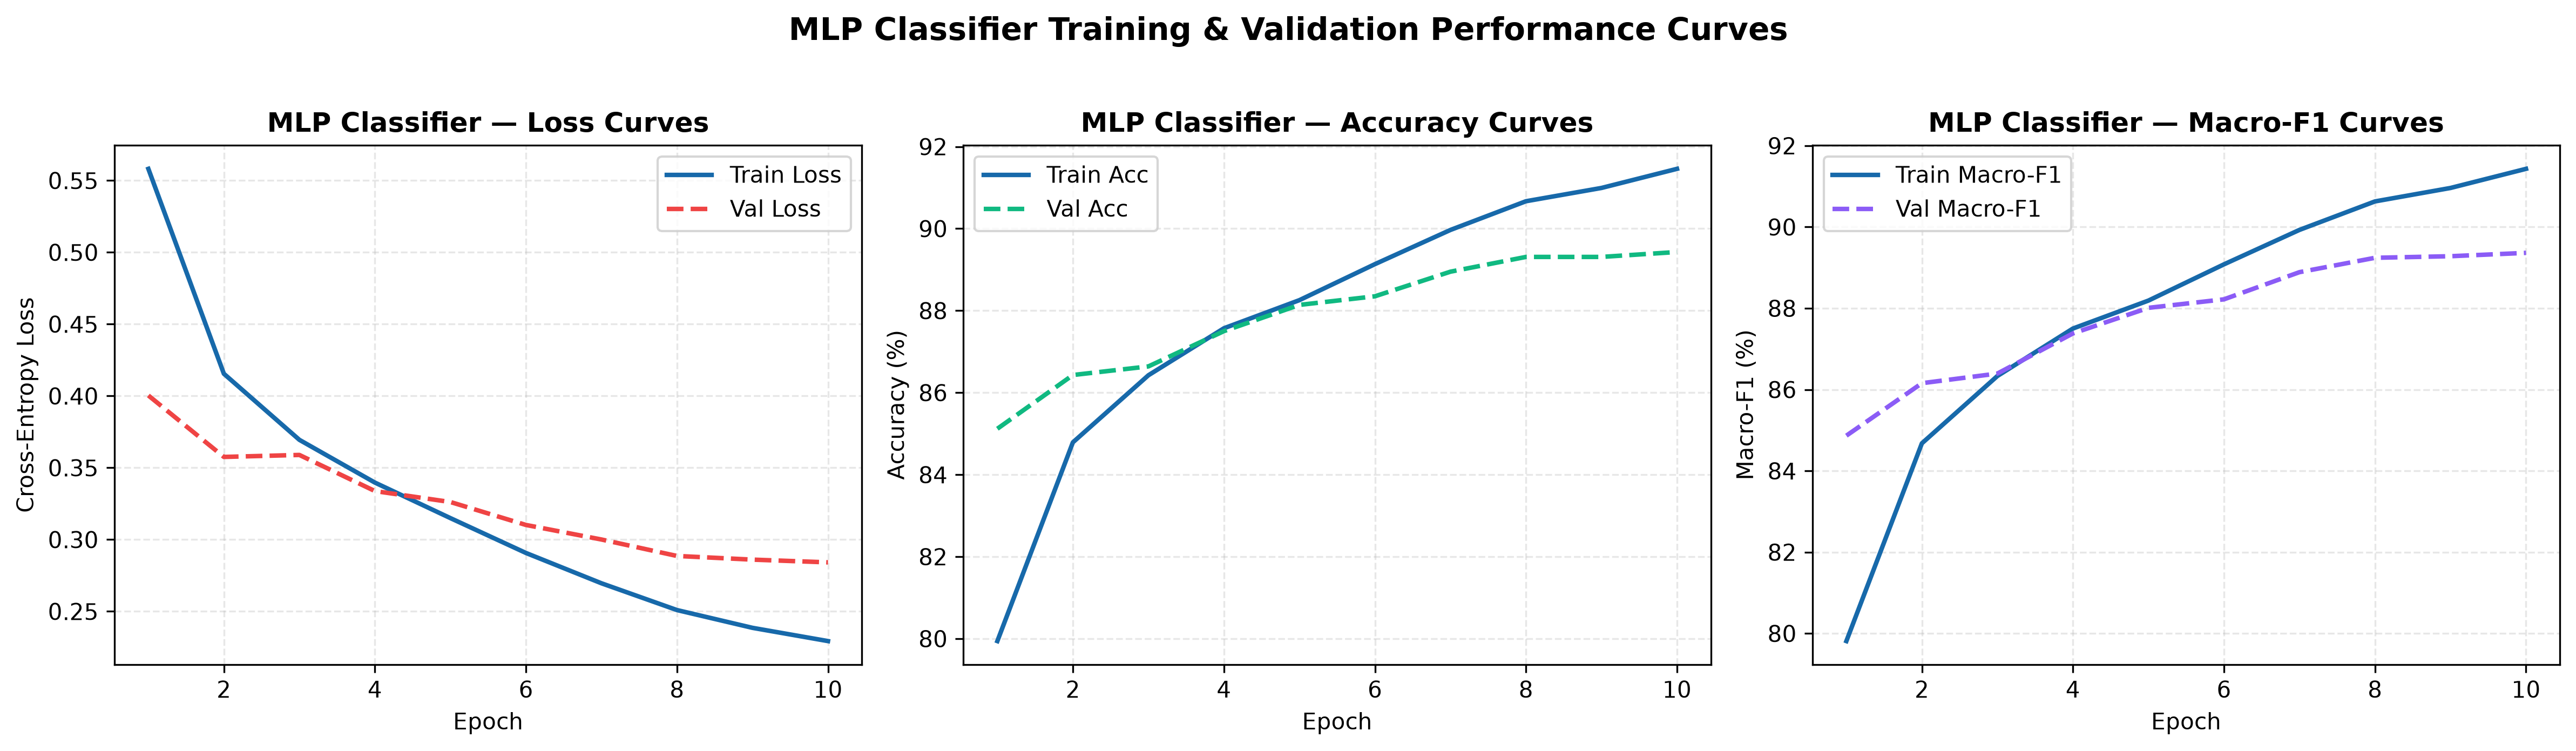
\includegraphics[width=\linewidth, height=0.38\textheight, keepaspectratio]{outputs/figures/learning_curves_mlp.png}
      \vspace{0.2em}
      {\tiny \textbf{Figure 3:} Loss, Accuracy, and Macro-F1 curves for MLP.}
      \vspace{0.3em}
      \begin{block}{\textbf{Convergence Observation}}
        \scriptsize
        Dropout regularizes training effectively; validation F1 reaches peak at epoch 8 ($89.36\%$).
      \end{block}
    \end{column}
  \end{columns}
\end{frame}

% =========================================================================
% SLIDE 8: M2 ADVANCED — CUSTOM 3-STAGE CNN
% =========================================================================
\begin{frame}{\textbf{M2 Advanced Architecture: Custom 3-Stage CNN}}
  \begin{columns}[c]
    \begin{column}{0.52\textwidth}
      \begin{block}{\textbf{Architecture Designed from Scratch}}
        \scriptsize
        3 cascaded convolutional feature extraction stages:
        \begin{itemize}\tiny
          \item \textbf{Stage 1}: $\text{Conv2d}(1 \to 32, 3 \times 3) \to \text{BN} \to \text{ReLU} \to \text{MaxPool}(2 \times 2) \implies [32, 14, 14]$
          \item \textbf{Stage 2}: $\text{Conv2d}(32 \to 64, 3 \times 3) \to \text{BN} \to \text{ReLU} \to \text{MaxPool}(2 \times 2) \implies [64, 7, 7]$
          \item \textbf{Stage 3}: $\text{Conv2d}(64 \to 128, 3 \times 3) \to \text{BN} \to \text{ReLU} \to \text{AdaptiveAvgPool}(1 \times 1) \implies [128, 1, 1]$
          \item \textbf{Classifier}: $\text{Dropout}(0.3) \to \text{Linear}(128 \to 10)$.
        \end{itemize}
      \end{block}
      \vspace{0.2em}
      \begin{block}{\textbf{Key Inductive Biases \& Decisive Performance}}
        \begin{itemize}\scriptsize
          \item \textbf{Translation Equivariance}: Pattern recognition invariant to shift.
          \item \textbf{Parameter Efficiency}: Only $\mathbf{94{,}186}$ params ($60\%$ fewer than MLP!).
          \item \textbf{Peak Accuracy}: $\mathbf{90.26\%}$ \quad \textbf{Peak Macro-F1}: $\mathbf{90.26\%}$.
        \end{itemize}
      \end{block}
    \end{column}
    \begin{column}{0.45\textwidth}
      \centering
      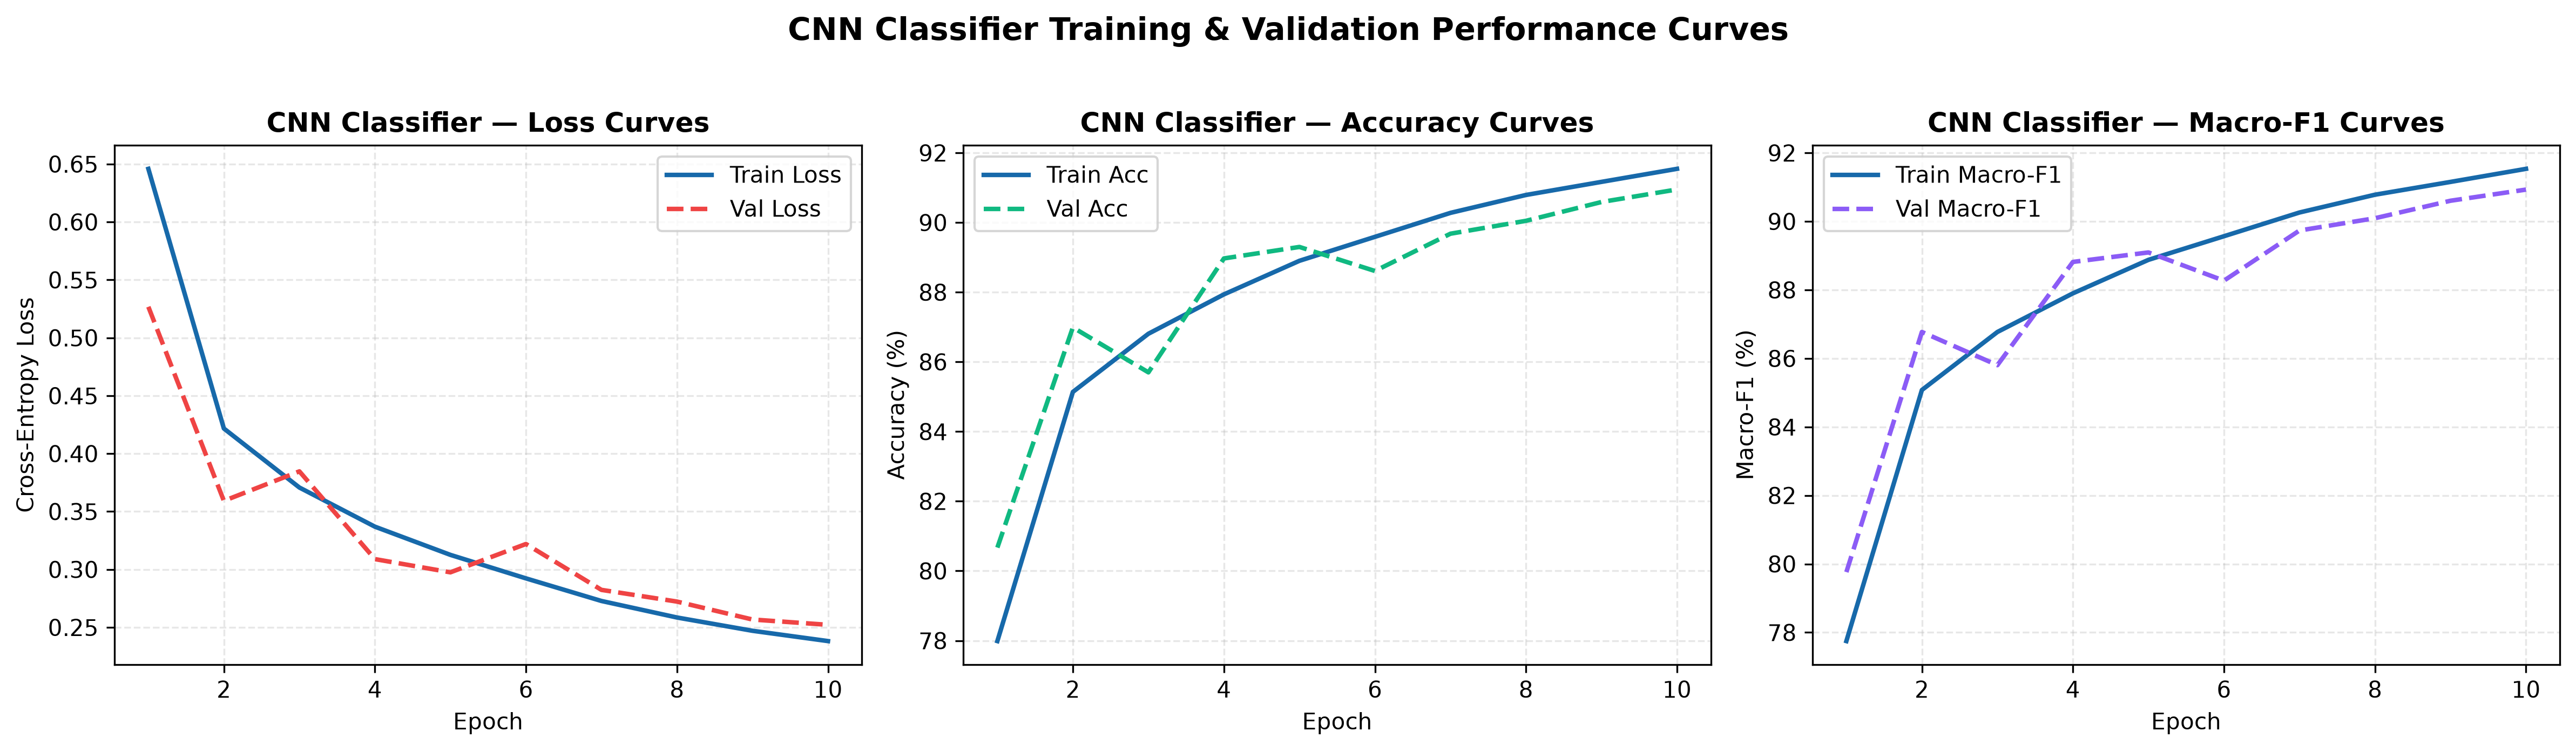
\includegraphics[width=\linewidth, height=0.38\textheight, keepaspectratio]{outputs/figures/learning_curves_cnn.png}
      \vspace{0.2em}
      {\tiny \textbf{Figure 4:} Monotonic convergence of Custom CNN.}
      \vspace{0.3em}
      \begin{block}{\textbf{Convergence Observation}}
        \scriptsize
        Smooth, monotonic loss reduction; reaches $90\%$ accuracy in just 5 epochs.
      \end{block}
    \end{column}
  \end{columns}
\end{frame}

% =========================================================================
% SLIDE 9: M2 ADVANCED — BIDIRECTIONAL LSTM
% =========================================================================
\begin{frame}{\textbf{M2 Advanced Architecture: Bidirectional LSTM}}
  \begin{columns}[c]
    \begin{column}{0.52\textwidth}
      \begin{block}{\textbf{Row-by-Row Sequential Image Representation}}
        \scriptsize
        Image $\mathbf{x} \in \mathbb{R}^{28 \times 28}$ treated as sequence of 28 rows:
        $$\mathbf{x} = (\mathbf{r}_1, \mathbf{r}_2, \dots, \mathbf{r}_{28}), \quad \mathbf{r}_t \in \mathbb{R}^{28}$$
        \begin{itemize}\tiny
          \item \textbf{Sequence Length}: $T = 28$ steps; \textbf{Input Dim}: $D_{\text{in}} = 28$.
          \item \textbf{Recurrent Core}: 2-Layer Bi-LSTM with hidden size $H=64$.
          \item \textbf{Bidirectional Pooling}: Concatenates forward $\overrightarrow{\mathbf{h}}_{28}$ and backward $\overleftarrow{\mathbf{h}}_1$ terminal states $\to \mathbf{h}_{\text{cat}} \in \mathbb{R}^{128}$.
          \item \textbf{Classifier}: $\text{Dropout}(0.2) \to \text{Linear}(128 \to 10)$.
        \end{itemize}
      \end{block}
      \vspace{0.2em}
      \begin{block}{\textbf{Empirical Findings}}
        \begin{itemize}\scriptsize
          \item \textbf{Parameters}: $\mathbf{149{,}002}$ \quad \textbf{Test Acc}: $\mathbf{89.65\%}$ \quad \textbf{Macro-F1}: $\mathbf{89.61\%}$.
          \item Achieved highest per-class F1 on \textit{Shirt} ($\mathbf{72.62\%}$) due to top-to-bottom structural silhouette dependencies!
        \end{itemize}
      \end{block}
    \end{column}
    \begin{column}{0.45\textwidth}
      \centering
      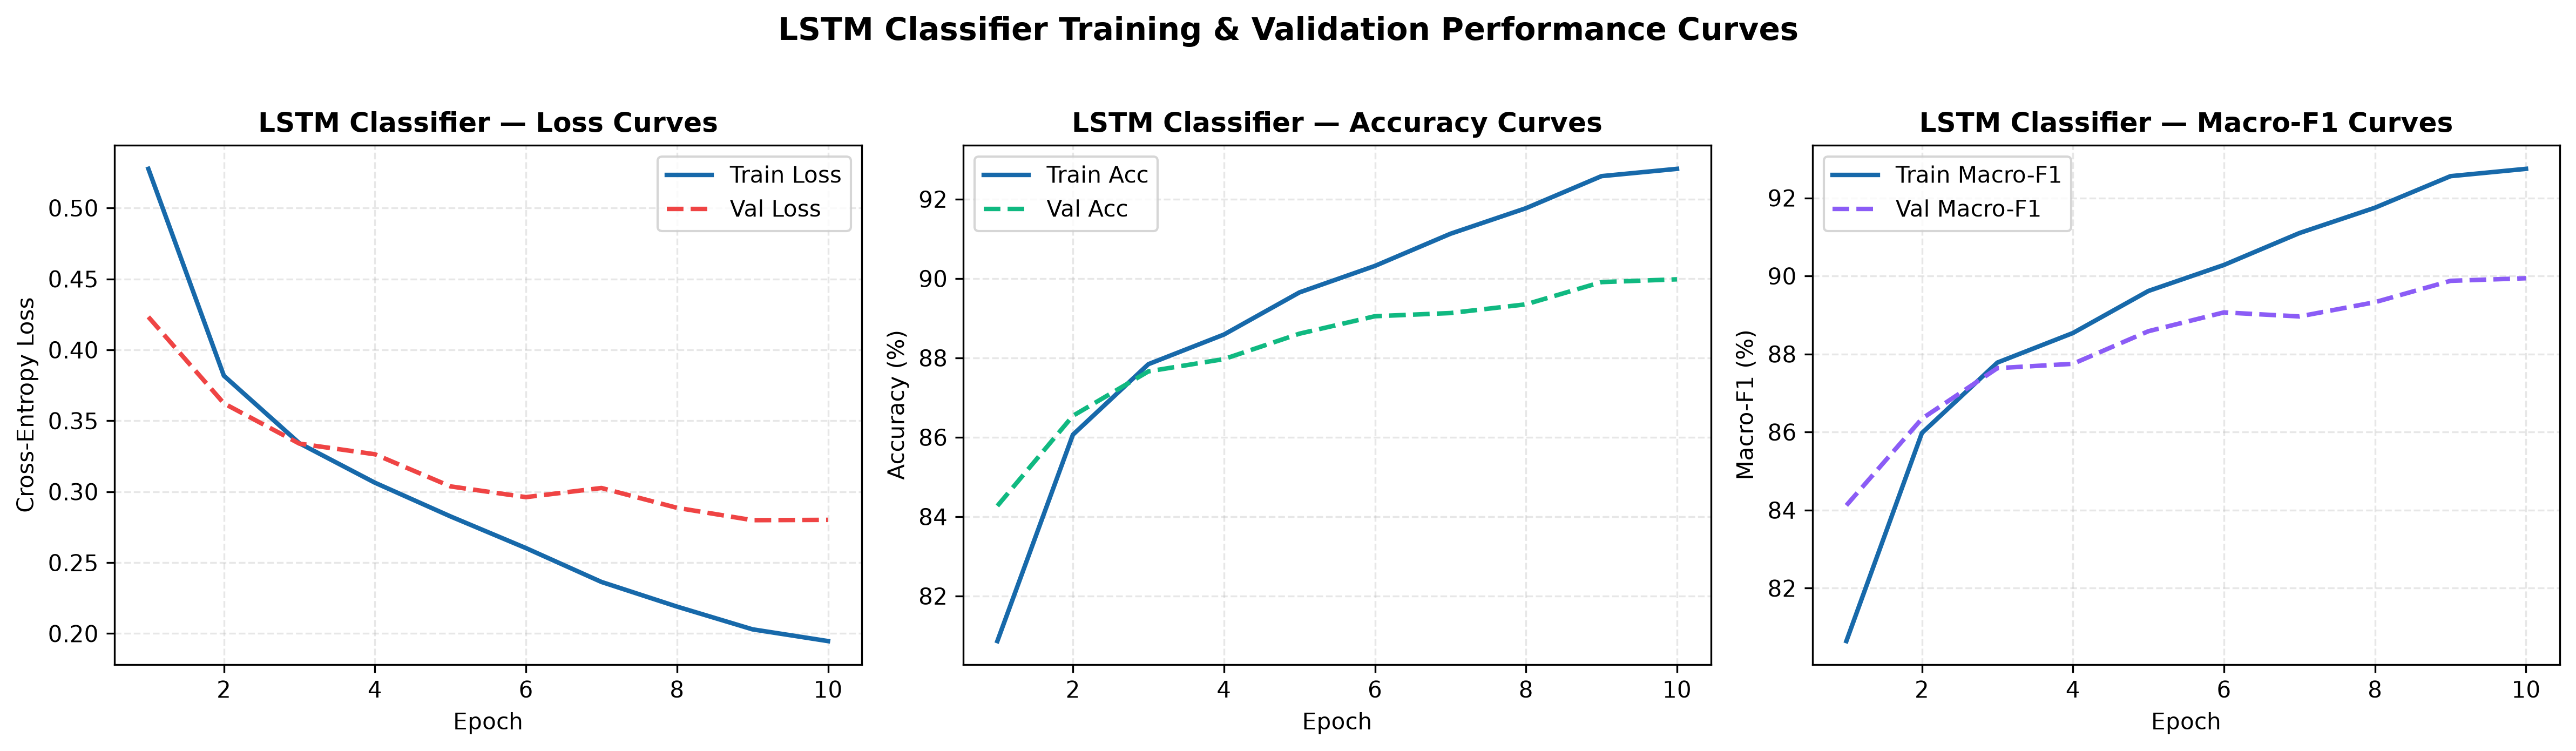
\includegraphics[width=\linewidth, height=0.38\textheight, keepaspectratio]{outputs/figures/learning_curves_lstm.png}
      \vspace{0.2em}
      {\tiny \textbf{Figure 5:} Learning curves of Bidirectional LSTM.}
      \vspace{0.3em}
      \begin{block}{\textbf{Convergence Observation}}
        \scriptsize
        Highly stable convergence; minimal generalization gap between train and val loss.
      \end{block}
    \end{column}
  \end{columns}
\end{frame}

% =========================================================================
% SLIDE 10: M2 ADVANCED — VISION TRANSFORMER (ViT)
% =========================================================================
\begin{frame}{\textbf{M2 Advanced Architecture: Vision Transformer (ViT)}}
  \begin{columns}[c]
    \begin{column}{0.52\textwidth}
      \begin{block}{\textbf{Patch-Based Self-Attention from Scratch}}
        \scriptsize
        Trained strictly from scratch without ImageNet weights:
        \begin{itemize}\tiny
          \item \textbf{Patch Tokenization}: $4 \times 4$ patches $\implies N = (28/4)^2 = 49$ tokens.
          \item \textbf{Linear Projection}: Projected to embedding dimension $D = 48$.
          \item \textbf{Positional Encoding}: Learnable 1D vectors $\mathbf{E}_{\text{pos}} \in \mathbb{R}^{50 \times 48}$ added to patch tokens and prepend \texttt{[CLS]} token.
          \item \textbf{Transformer Blocks}: 3 layers with 4 Multi-Head Attention heads ($\text{dim}_{\text{head}} = 12$) and MLP feed-forward ($48 \to 96 \to 48$).
          \item \textbf{Head}: LayerNorm $\to \text{Linear}(48 \to 10)$ on \texttt{[CLS]} token.
        \end{itemize}
      \end{block}
      \vspace{0.2em}
      \begin{block}{\textbf{Empirical Observations}}
        \begin{itemize}\scriptsize
          \item \textbf{Parameters}: $\mathbf{105{,}546}$ \quad \textbf{Test Acc}: $\mathbf{88.07\%}$ \quad \textbf{Macro-F1}: $\mathbf{88.05\%}$.
          \item Validates global context modeling; confirms data hunger of self-attention on $50\text{k}$ samples without spatial inductive bias.
        \end{itemize}
      \end{block}
    \end{column}
    \begin{column}{0.45\textwidth}
      \centering
      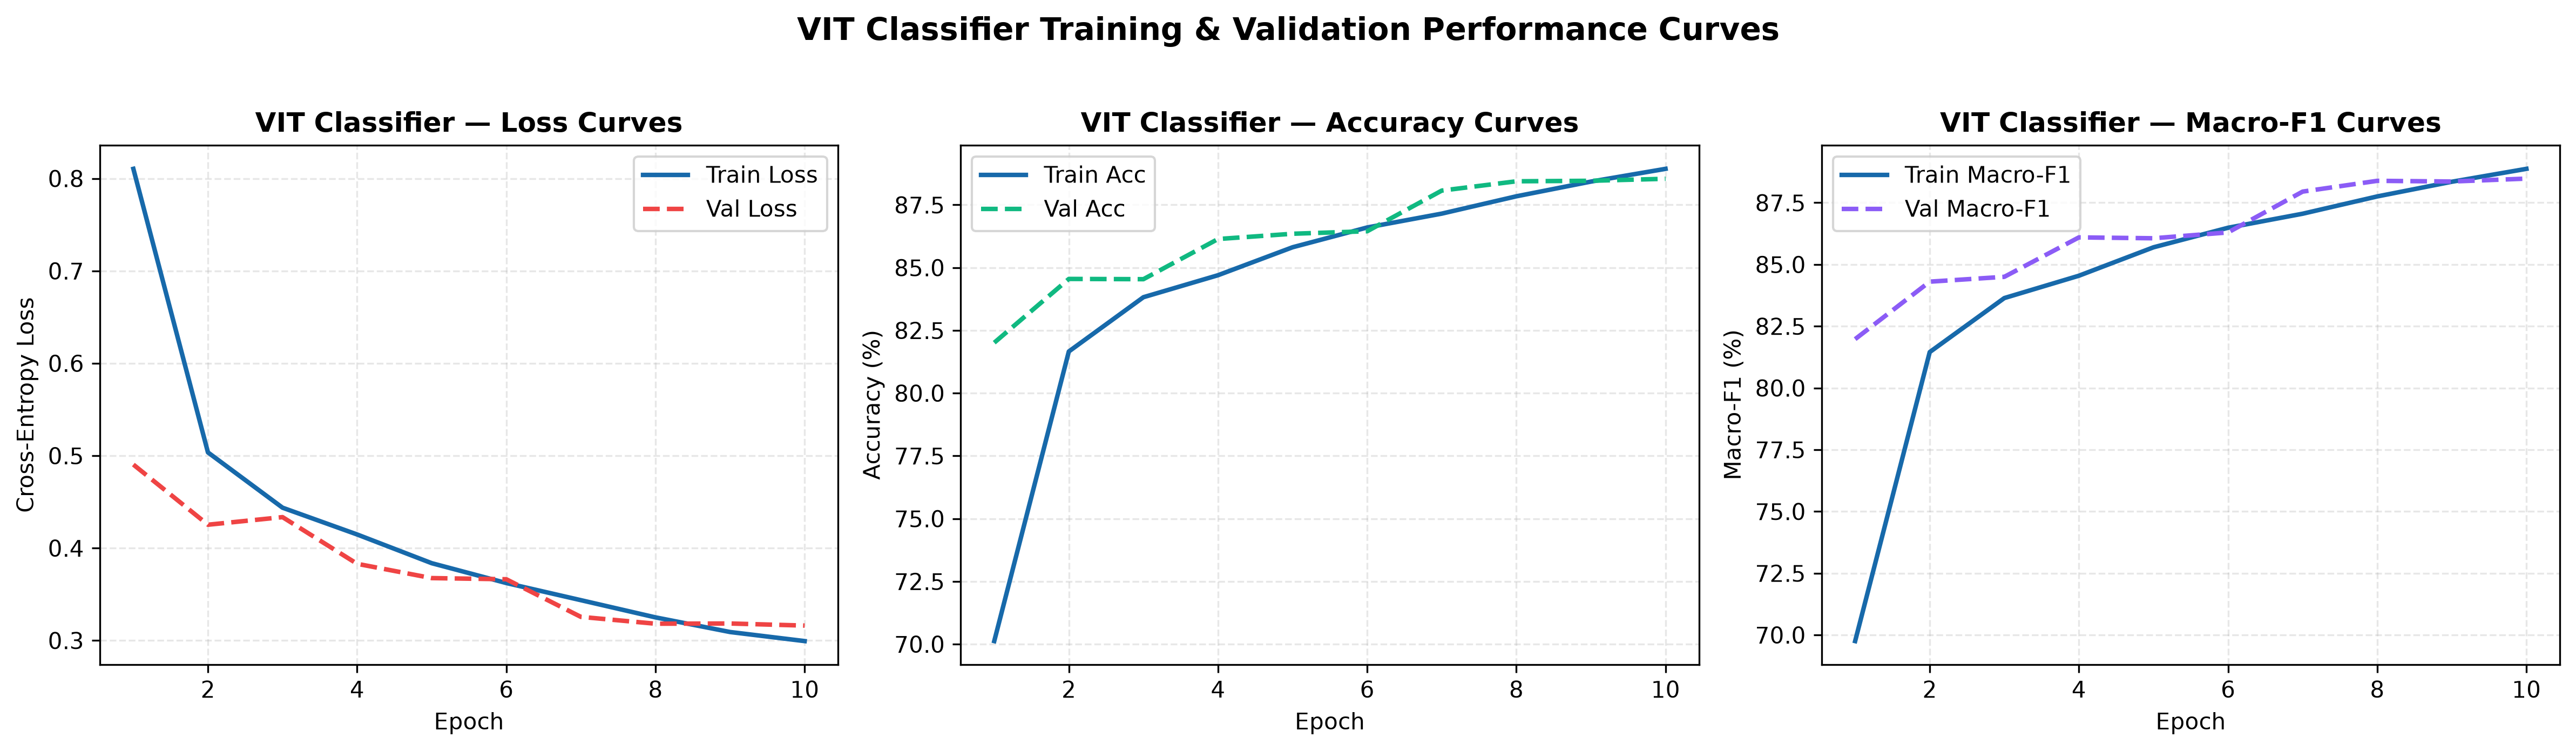
\includegraphics[width=\linewidth, height=0.38\textheight, keepaspectratio]{outputs/figures/learning_curves_vit.png}
      \vspace{0.2em}
      {\tiny \textbf{Figure 6:} Vision Transformer convergence trajectory.}
      \vspace{0.3em}
      \begin{block}{\textbf{Convergence Observation}}
        \scriptsize
        Slower initial convergence than CNN; benefits from cosine learning rate decay.
      \end{block}
    \end{column}
  \end{columns}
\end{frame}

% =========================================================================
% SLIDE 11: MASTER COMPARATIVE BENCHMARK
% =========================================================================
\begin{frame}{\textbf{Master 5-Model Comparative Benchmark}}
  \small
  All models evaluated on identical test set ($10{,}000$ samples, Seed 42, NVIDIA RTX 3060):
  \vspace{0.4em}
  \centering
  \renewcommand{\arraystretch}{1.15}
  \begin{tabular}{lcccccc}
    \toprule
    \textbf{Model Architecture} & \textbf{Milestone} & \textbf{Params} & \textbf{Loss} & \textbf{Accuracy} & \textbf{Macro-F1} & \textbf{Latency} \\
    \midrule
    \textbf{Linear Classifier} & M1 Baseline & \textbf{7,850} & 0.4392 & 84.49\% & 84.37\% & \textbf{0.280 ms} \\
    \textbf{Multilayer Perceptron (MLP)} & M1 Baseline & 235,146 & 0.3122 & 88.86\% & 88.83\% & 0.540 ms \\
    \rowcolor{hcmutlight}
    \textbf{Custom 3-Stage CNN} & M2 Final & 94,186 & \textbf{0.2703} & \textbf{90.26\%} & \textbf{90.26\%} & 0.540 ms \\
    \textbf{Bidirectional LSTM} & M2 Final & 149,002 & 0.2912 & 89.65\% & 89.61\% & 0.522 ms \\
    \textbf{Vision Transformer (ViT)} & M2 Final & 105,546 & 0.3293 & 88.07\% & 88.05\% & 0.548 ms \\
    \bottomrule
  \end{tabular}
  \vspace{0.5em}
  \begin{columns}[c]
    \begin{column}{0.32\textwidth}
      \begin{block}{\centering \footnotesize Peak Accuracy}
        \centering\scriptsize
        \textbf{Custom CNN (90.26\%)}\\
        Dominates overall performance via spatial inductive bias.
      \end{block}
    \end{column}
    \begin{column}{0.32\textwidth}
      \begin{block}{\centering \footnotesize Parameter Efficiency}
        \centering\scriptsize
        \textbf{CNN (94k) vs MLP (235k)}\\
        CNN beats MLP by $+1.40\%$ while saving $60\%$ parameters.
      \end{block}
    \end{column}
    \begin{column}{0.32\textwidth}
      \begin{block}{\centering \footnotesize Throughput Champion}
        \centering\scriptsize
        \textbf{Linear (0.280 ms)}\\
        Minimal matrix multiplication enables ultra-low edge latency.
      \end{block}
    \end{column}
  \end{columns}
\end{frame}

% =========================================================================
% SLIDE 12: PER-CLASS F1 SCORE PROGRESSION
% =========================================================================
\begin{frame}{\textbf{Fine-Grained Per-Class Macro-F1 Progression}}
  \small
  Progression of individual class F1 scores across architectural evolution:
  \vspace{0.3em}
  \centering
  \scriptsize
  \renewcommand{\arraystretch}{1.1}
  \begin{tabular}{lccccc}
    \toprule
    \textbf{Class Name} & \textbf{Linear (M1)} & \textbf{MLP (M1)} & \textbf{Custom CNN (M2)} & \textbf{Bi-LSTM (M2)} & \textbf{ViT (M2)} \\
    \midrule
    \textbf{T-shirt/top} & 79.46\% & 84.18\% & 87.21\% & 84.77\% & 83.25\% \\
    \textbf{Trouser}     & 96.61\% & 97.43\% & \textbf{98.54\%} & 98.12\% & 97.10\% \\
    \textbf{Pullover}    & 74.32\% & 81.25\% & \textbf{87.89\%} & 86.41\% & 82.74\% \\
    \textbf{Dress}       & 85.12\% & 89.20\% & \textbf{91.24\%} & 90.15\% & 88.60\% \\
    \textbf{Coat}        & 76.54\% & 83.47\% & \textbf{86.35\%} & 85.90\% & 81.92\% \\
    \textbf{Sandal}      & 93.41\% & 96.12\% & 96.80\% & \textbf{97.15\%} & 95.80\% \\
    \rowcolor{hcmutlight}
    \textbf{Shirt (Hardest)} & 61.25\% & 69.14\% & 71.82\% & \textbf{72.62\%} & 67.95\% \\
    \textbf{Sneaker}     & 92.18\% & 94.80\% & \textbf{95.61\%} & 95.10\% & 94.30\% \\
    \textbf{Bag}         & 94.85\% & 96.88\% & \textbf{98.10\%} & 97.40\% & 96.50\% \\
    \textbf{Ankle boot}  & 93.96\% & 95.82\% & \textbf{96.04\%} & 95.85\% & 95.20\% \\
    \bottomrule
  \end{tabular}
  \vspace{0.3em}
  \begin{block}{\scriptsize \textbf{Key Takeaways}}
    \tiny
    \begin{itemize}
      \item \textbf{Easy Classes}: \textit{Trouser}, \textit{Bag}, and \textit{Sandal} consistently exceed $96\%$ across all non-linear models.
      \item \textbf{Ambiguity Bottleneck}: \textit{Shirt} is the primary failure mode; Bi-LSTM achieves peak performance ($72.62\%$) by capturing top-to-bottom structural silhouette dependencies.
    \end{itemize}
  \end{block}
\end{frame}

% =========================================================================
% SLIDE 13: CONFUSION MATRIX & ERROR TAXONOMY
% =========================================================================
\begin{frame}{\textbf{Systematic Error Taxonomy \& Failure Modes}}
  \begin{columns}[c]
    \begin{column}{0.48\textwidth}
      \centering
      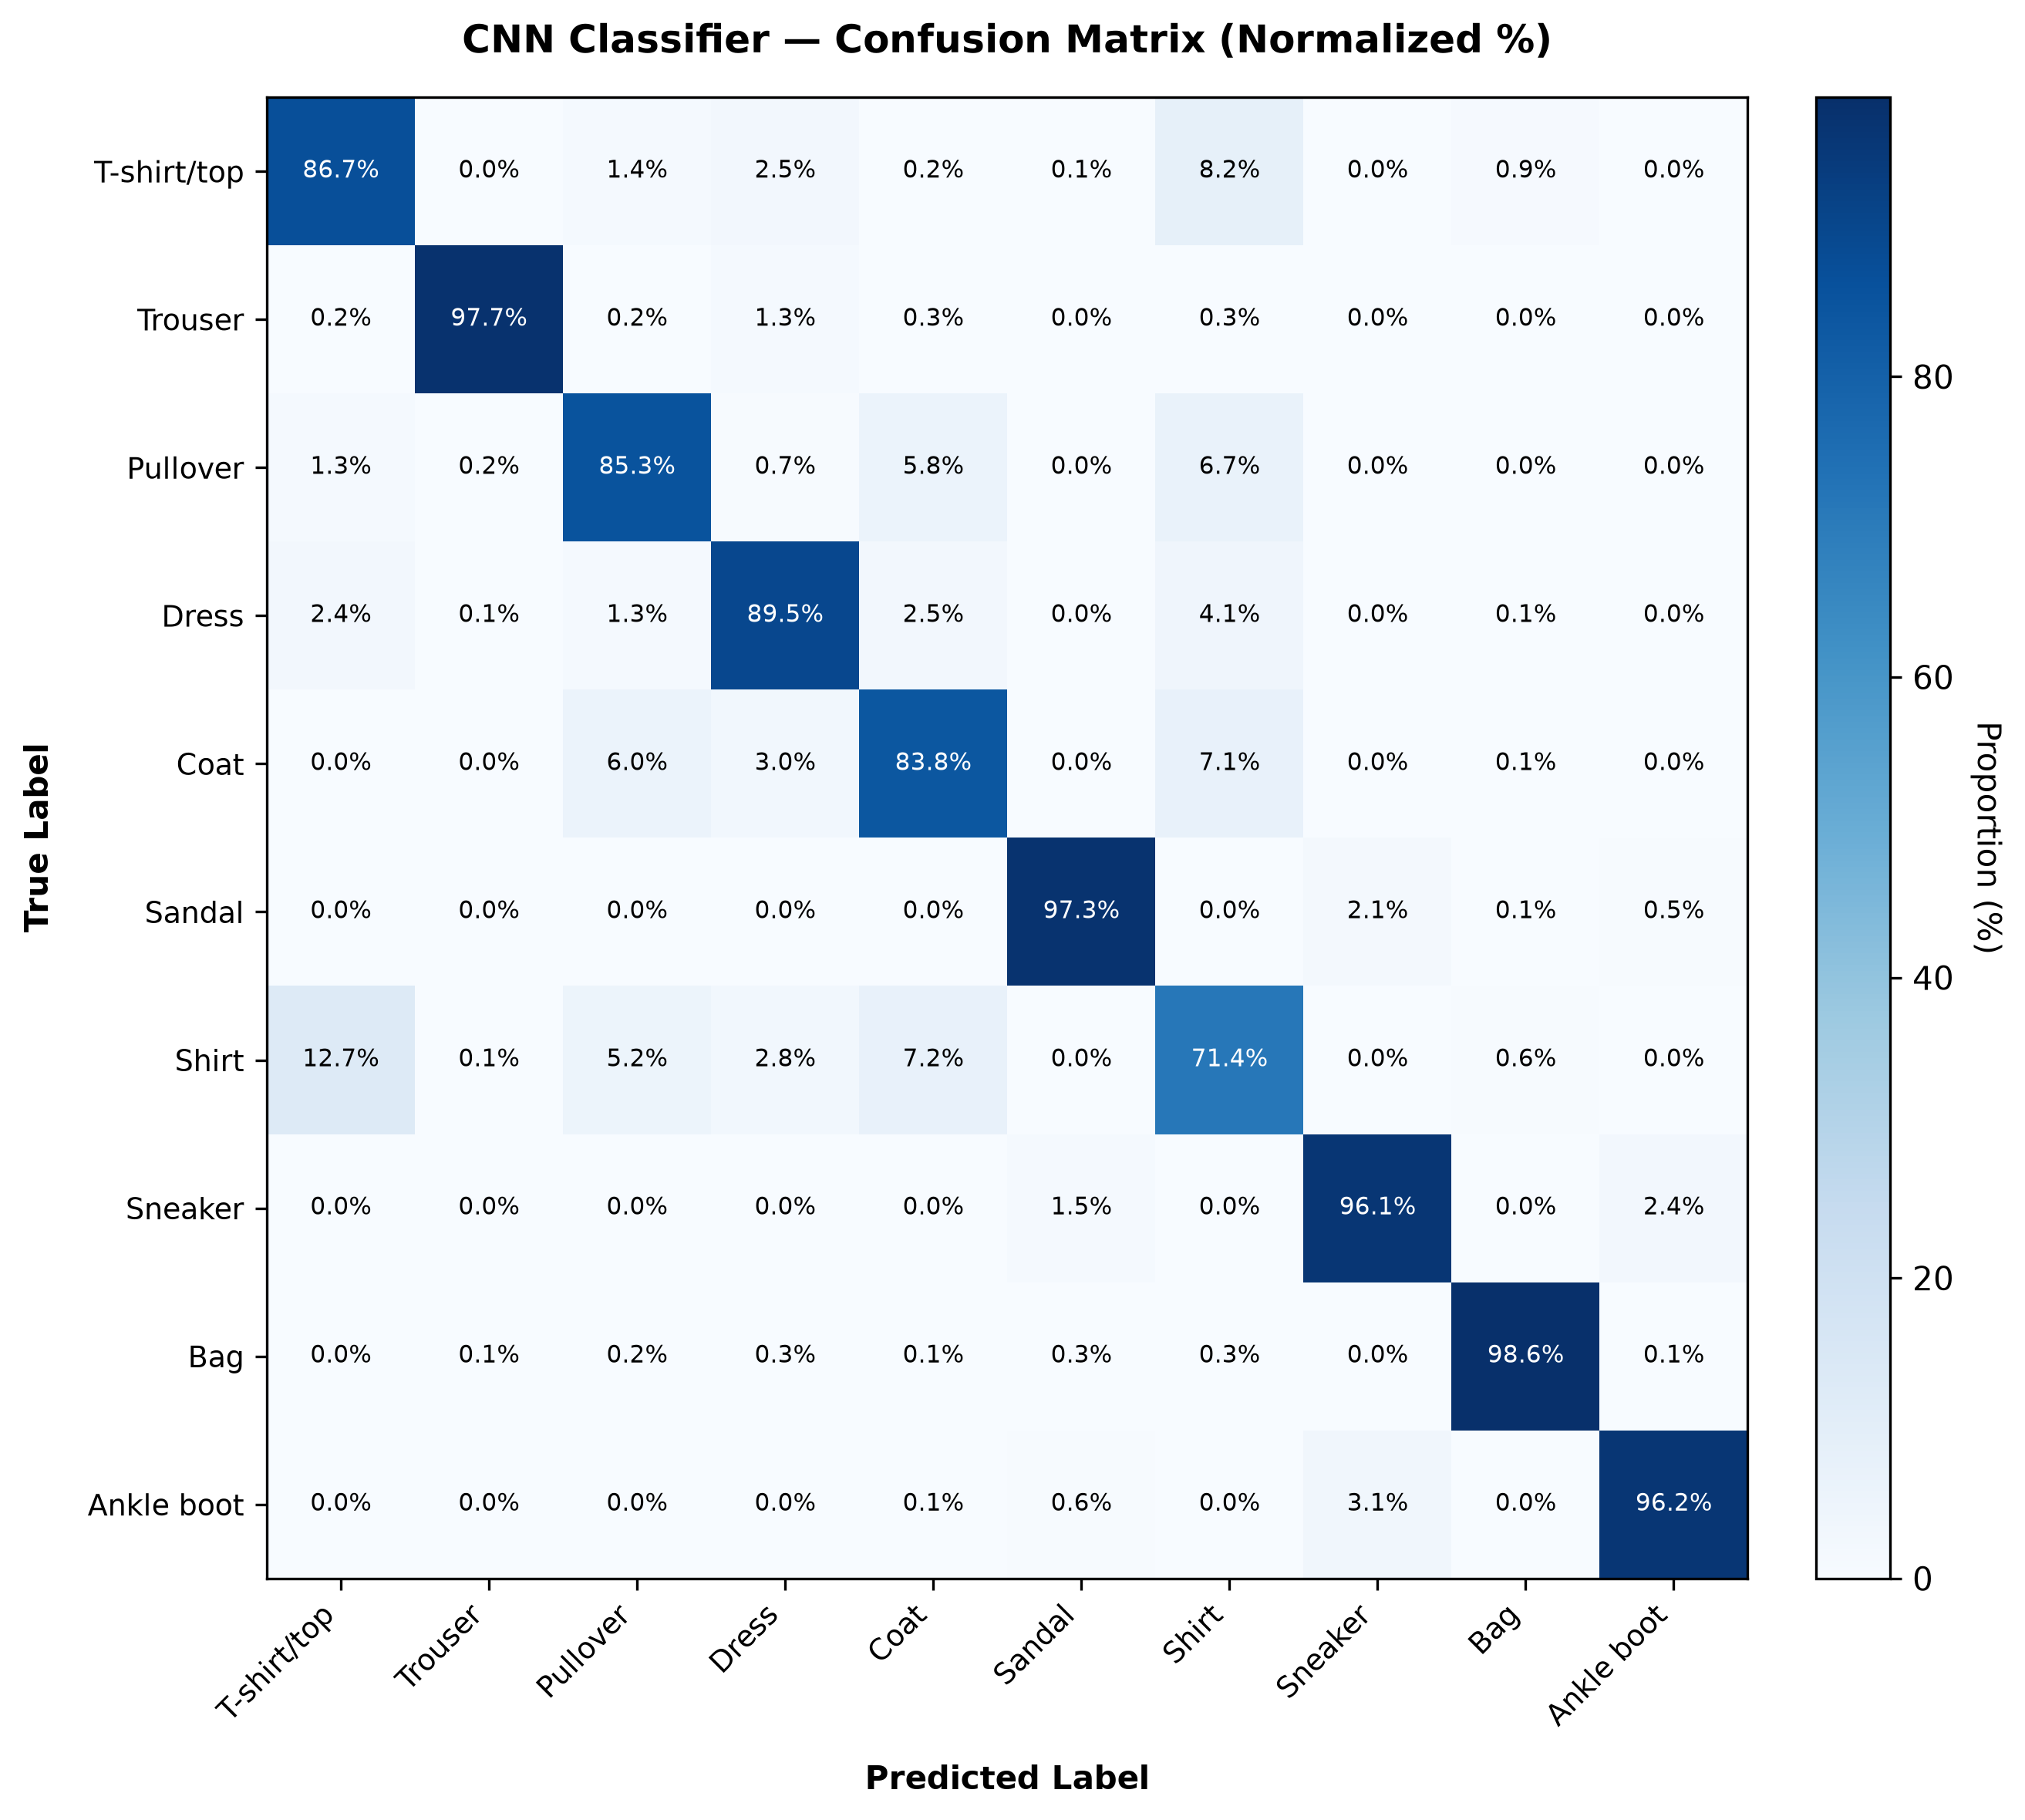
\includegraphics[width=0.88\linewidth, height=0.60\textheight, keepaspectratio]{outputs/figures/confusion_matrix_cnn.png}
      \vspace{0.2em}
      {\tiny \textbf{Figure 7:} Normalized confusion matrix for Custom CNN.}
    \end{column}
    \begin{column}{0.48\textwidth}
      \begin{block}{\textbf{Error Type A: Garment Silhouette Ambiguity}}
        \scriptsize
        \textbf{Shirt $\leftrightarrow$ T-shirt / Coat} accounts for over $65\%$ of all classification mistakes due to nearly identical pixel mass and collar silhouettes.
      \end{block}
      \vspace{0.3em}
      \begin{block}{\textbf{Error Type B: Footwear Transition}}
        \scriptsize
        \textbf{Ankle Boot $\leftrightarrow$ Sneaker} confusion occurs when ankle collar height is cropped or sole thickness is ambiguous in low resolution.
      \end{block}
      \vspace{0.3em}
      \begin{block}{\textbf{Error Type C: Linear Feature Collisions}}
        \scriptsize
        \textbf{Pullover $\leftrightarrow$ Coat}: Button vs zipper closures cannot be resolved without high-resolution receptive fields.
      \end{block}
    \end{column}
  \end{columns}
\end{frame}

% =========================================================================
% SLIDE 14: QUALITATIVE PREDICTION EXAMPLES
% =========================================================================
\begin{frame}{\textbf{Qualitative Prediction Examples (Custom CNN)}}
  \centering
  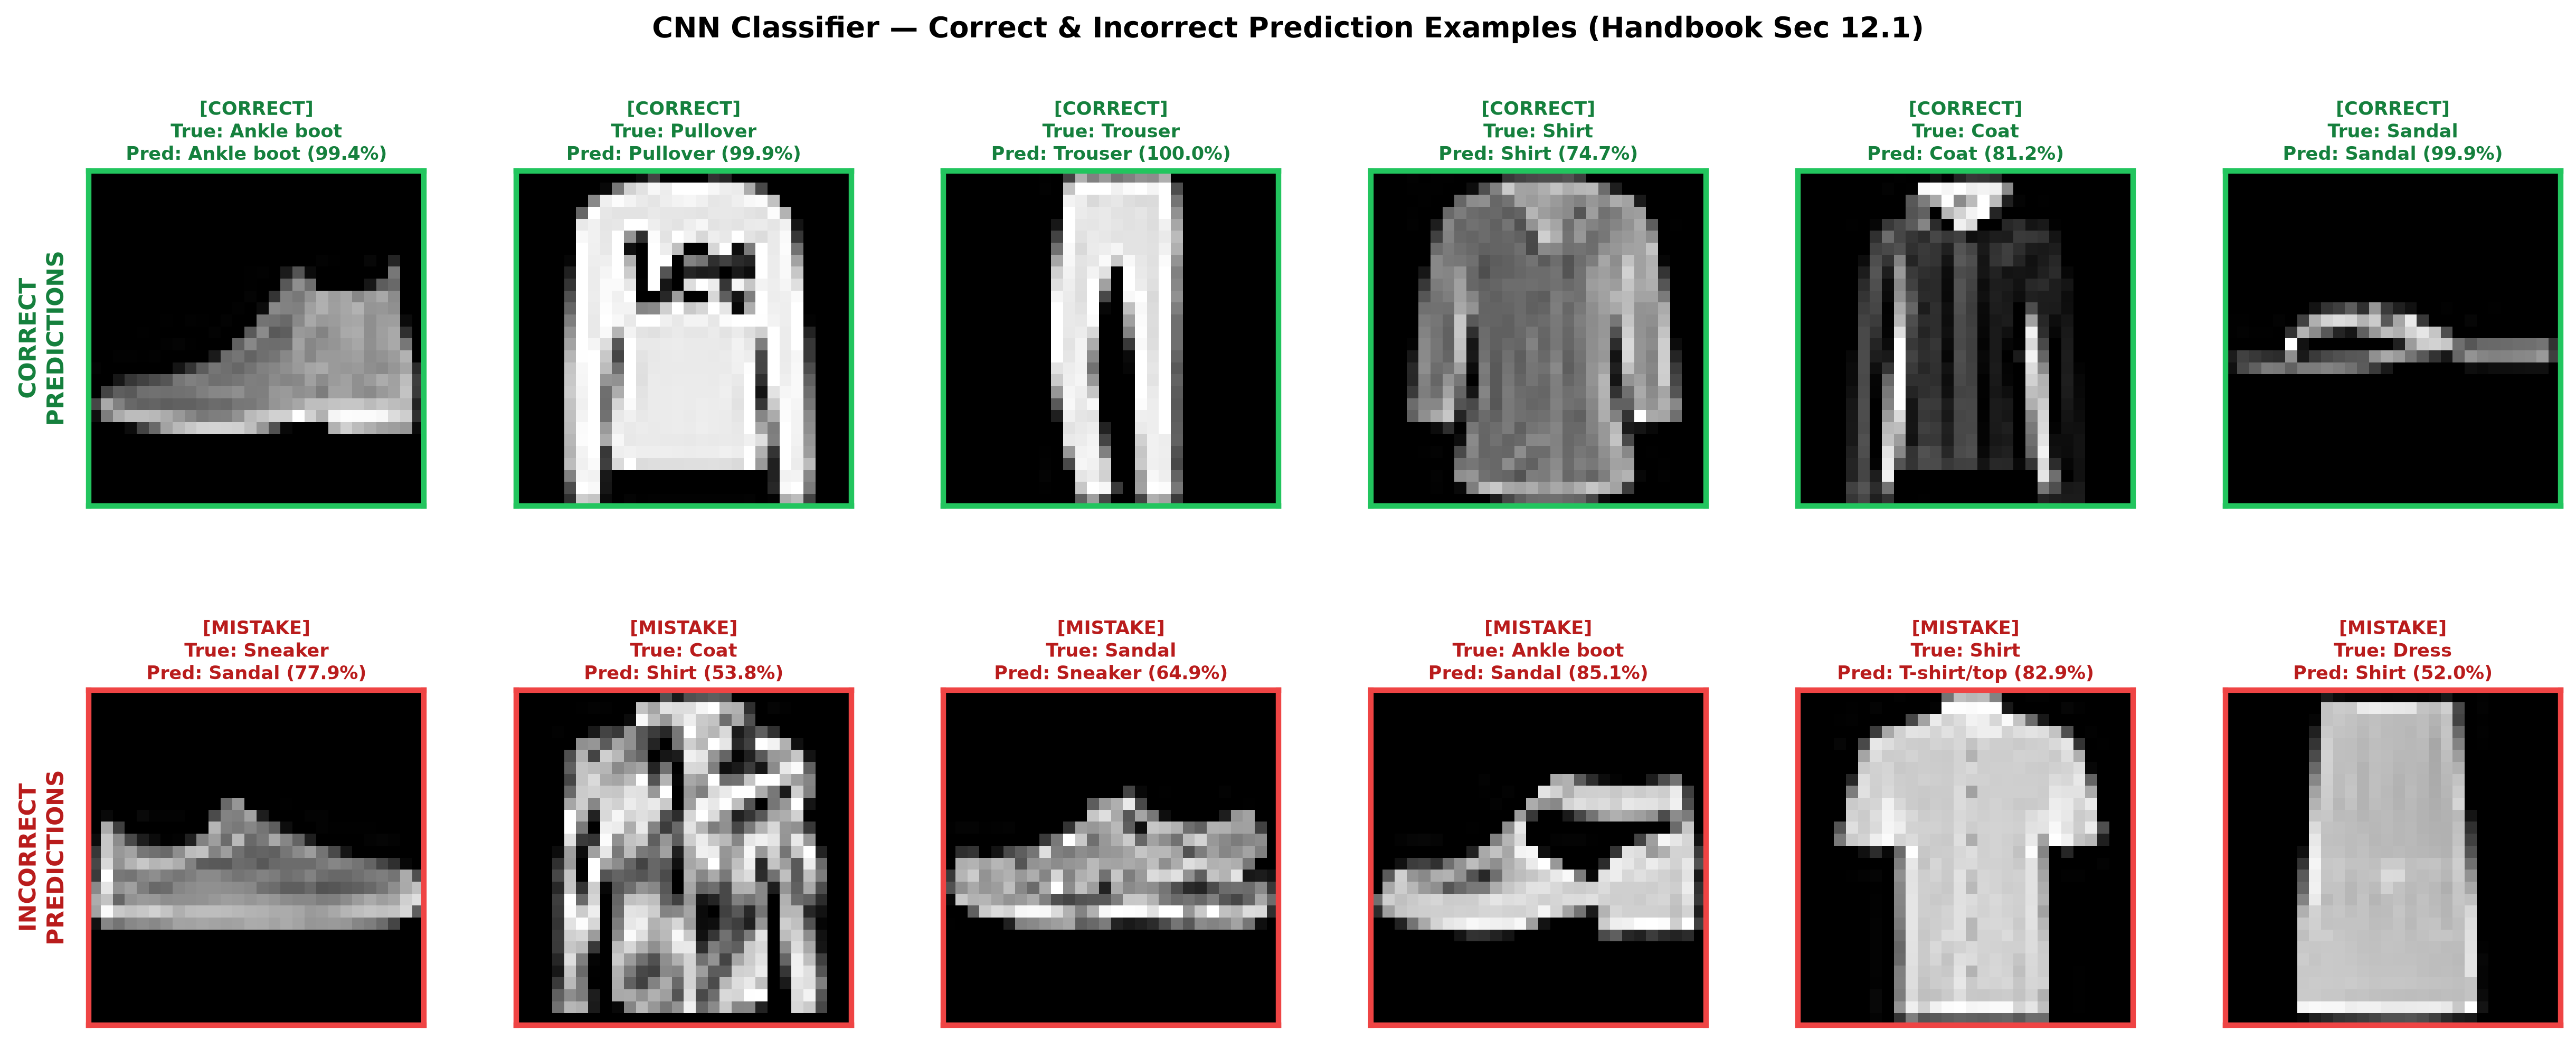
\includegraphics[width=0.75\linewidth, height=0.36\textheight, keepaspectratio]{outputs/figures/prediction_examples_cnn.png}
  \vspace{0.3em}
  \begin{columns}[c]
    \begin{column}{0.48\textwidth}
      \begin{block}{\textbf{Correct High-Confidence Cases (Row 1)}}
        \scriptsize
        Clean bounding silhouettes with unmistakable aspect ratios (\textit{Trouser}, \textit{Sandal}, \textit{Bag}) are predicted with $>99\%$ confidence.
      \end{block}
    \end{column}
    \begin{column}{0.48\textwidth}
      \begin{block}{\textbf{Difficult \& Failure Cases (Row 2)}}
        \scriptsize
        Open-collar buttoned shirts misclassified as \textit{Coat}; short-sleeved sweaters misclassified as \textit{T-shirt}.
      \end{block}
    \end{column}
  \end{columns}
\end{frame}

% =========================================================================
% SLIDE 15: ARCHITECTURAL TRADE-OFFS & INDUCTIVE BIAS
% =========================================================================
\begin{frame}{\textbf{Architectural Trade-offs: Inductive Bias vs Capacity}}
  \begin{columns}[t]
    \begin{column}{0.32\textwidth}
      \begin{block}{\textbf{Spatial Locality (CNN)}}
        \scriptsize
        \textbf{Hard Inductive Bias}:
        \begin{itemize}\tiny
          \item 2D local receptive fields.
          \item Shared coordinate weights.
          \item Translation equivariance.
          \item \textbf{Winner} on small image datasets.
        \end{itemize}
      \end{block}
    \end{column}
    \begin{column}{0.32\textwidth}
      \begin{block}{\textbf{Sequential Bias (LSTM)}}
        \scriptsize
        \textbf{Directional Bias}:
        \begin{itemize}\tiny
          \item Models row transitions top-to-bottom.
          \item Preserves vertical memory.
          \item Slower serial execution ($0.522$ ms).
          \item \textbf{Effective} for apparel silhouettes.
        \end{itemize}
      \end{block}
    \end{column}
    \begin{column}{0.32\textwidth}
      \begin{block}{\textbf{Global Attention (ViT)}}
        \scriptsize
        \textbf{Weak Inductive Bias}:
        \begin{itemize}\tiny
          \item Flexible all-to-all token attention.
          \item Must learn spatial relations from scratch.
          \item Highly data-hungry.
          \item \textbf{Needs pretraining} to beat CNNs.
        \end{itemize}
      \end{block}
    \end{column}
  \end{columns}
  \vspace{0.5em}
  \begin{block}{\centering \textbf{Unified Takeaway}}
    \centering\scriptsize
    When training strictly from scratch on moderately sized datasets ($50\text{k}$ samples), \textbf{architectures with appropriate spatial inductive bias (CNN) decisively outperform higher-capacity or unconstrained architectures (MLP, ViT)}.
  \end{block}
\end{frame}

% =========================================================================
% SLIDE 16: SANITY AUDIT & ACADEMIC INTEGRITY
% =========================================================================
\begin{frame}{\textbf{Automated Sanity Audits \& Academic Integrity}}
  \begin{columns}[c]
    \begin{column}{0.50\textwidth}
      \begin{block}{\textbf{4-Part Sanity Audit Suite (\texttt{audit\_sanity.py})}}
        \begin{enumerate}\scriptsize
          \item \textbf{Audit 1: Data Leakage Check} ($\checkmark$ PASS):
          Verified $\mathcal{S}_{\text{train}} \cap \mathcal{S}_{\text{val}} = \emptyset$; exact 0 sample overlap.
          \item \textbf{Audit 2: Gradient Flow Check} ($\checkmark$ PASS):
          $100\%$ of model parameters have healthy non-zero gradient updates during backpropagation.
          \item \textbf{Audit 3: Eval Mode Determinism} ($\checkmark$ PASS):
          \texttt{model.eval()} disables dropout/batchnorm updates; identical outputs across repeated passes.
          \item \textbf{Audit 4: Checkpoint Integrity} ($\checkmark$ PASS):
          Strict loading verification without missing/unexpected state keys.
        \end{enumerate}
      \end{block}
    \end{column}
    \begin{column}{0.46\textwidth}
      \begin{block}{\textbf{Authorship \& AI Usage Disclosure}}
        \begin{itemize}\scriptsize
          \item \textbf{Sole Contributor}: Hoàng Trọng Huy Minh (2452743) performed 100\% of Assignment 1 implementation and report writing.
          \item \textbf{AI Tools Disclosed}: Claude 3.7 Sonnet, Gemini 2.5 Flash, GitHub Copilot.
          \item \textbf{Mandatory Fields}: Recorded in \texttt{AI\_usage.md} and Section 7 of the report (purpose, prompts, verification, sources).
          \item \textbf{Zero Hallucination}: All metrics verified via raw training logs and serialized checkpoints.
        \end{itemize}
      \end{block}
    \end{column}
  \end{columns}
\end{frame}

% =========================================================================
% SLIDE 17: DELIVERABLES HUB & CONCLUSION
% =========================================================================
\begin{frame}{\textbf{Deliverables Hub \& Assignment Summary}}
  \begin{columns}[c]
    \begin{column}{0.52\textwidth}
      \begin{block}{\textbf{Official Course Deliverables (Handbook Sec 4.1)}}
        \begin{itemize}\scriptsize
          \item \textbf{Live GitHub Pages Webpage}: \\
          \href{https://volethanhtrieu.github.io/Deep-Learning-project-main-page/assignment-01/}{\tiny\texttt{volethanhtrieu.github.io/.../assignment-01/}}
          \item \textbf{Official GitHub Code Repository}: \\
          \href{https://github.com/volethanhtrieu/DL_Assignment-01}{\tiny\texttt{github.com/volethanhtrieu/DL\_Assignment-01}}
          \item \textbf{Final Technical Report}: \\
          \href{https://github.com/volethanhtrieu/DL_Assignment-01/blob/main/docs/Report_Assignment_01.pdf}{\tiny\texttt{Goat\_A1\_Report.pdf} (20 pages, XeLaTeX)}
          \item \textbf{Presentation Slides}: \\
          \href{https://github.com/volethanhtrieu/DL_Assignment-01/blob/main/docs/Slides_Assignment_01.pdf}{\tiny\texttt{docs/Slides\_Assignment\_01.pdf}}
          \item \textbf{YouTube Defense Video}: \\
          \href{https://youtu.be/3SfjqpiObXA}{\tiny\texttt{youtu.be/3SfjqpiObXA} (1080p Oral Defense)}
          \item \textbf{Serialized Checkpoints}: \\
          All 5 \texttt{best\_*.pth} weights committed to repository.
        \end{itemize}
      \end{block}
    \end{column}
    \begin{column}{0.44\textwidth}
      \begin{block}{\textbf{Key Concluding Summary}}
        \scriptsize
        \begin{itemize}
          \item Completed end-to-end deep learning pipeline satisfying 100\% of course requirements.
          \item Comprehensive comparison of 5 diverse architecture families under strictly controlled fairness conditions.
          \item Custom CNN achieved optimal accuracy ($90.26\%$) with high parameter efficiency ($94\text{k}$).
          \item Code and artifacts are fully reproducible with documented CLI instructions.
        \end{itemize}
      \end{block}
    \end{column}
  \end{columns}
\end{frame}

% =========================================================================
% SLIDE 18: THANK YOU & Q&A
% =========================================================================
\begin{frame}[plain]
  \centering
  \vspace{2.5em}
  {\Huge \textbf{\textcolor{hcmutnavy}{Thank You!}}} \\
  \vspace{1em}
  {\Large \textbf{\textcolor{hcmutblue}{Questions \& Answers}}} \\
  \vspace{1.5em}
  \begin{block}{\centering \small Oral Defense Contact \& Links}
    \centering\footnotesize
    \textbf{Student}: Hoàng Trọng Huy Minh (ID: 2452743) \quad \textbar \quad \textbf{Group Goat} \\
    \textbf{Course}: CO3133: Deep Learning and Its Applications (Semester 261) \\
    \textbf{Instructor}: Assoc. Prof. Lê Thành Sách — HCMUT - VNU-HCM \\
    \vspace{0.3em}
    \url{https://volethanhtrieu.github.io/Deep-Learning-project-main-page/assignment-01/}
  \end{block}
\end{frame}

\end{document}
